\documentclass[11pt,]{article}
\usepackage[]{mathpazo}
\usepackage{amssymb,amsmath}
\usepackage{ifxetex,ifluatex}
\usepackage{fixltx2e} % provides \textsubscript
\ifnum 0\ifxetex 1\fi\ifluatex 1\fi=0 % if pdftex
  \usepackage[T1]{fontenc}
  \usepackage[utf8]{inputenc}
\else % if luatex or xelatex
  \ifxetex
    \usepackage{mathspec}
  \else
    \usepackage{fontspec}
  \fi
  \defaultfontfeatures{Ligatures=TeX,Scale=MatchLowercase}
\fi
% use upquote if available, for straight quotes in verbatim environments
\IfFileExists{upquote.sty}{\usepackage{upquote}}{}
% use microtype if available
\IfFileExists{microtype.sty}{%
\usepackage{microtype}
\UseMicrotypeSet[protrusion]{basicmath} % disable protrusion for tt fonts
}{}
\usepackage[margin = 1in]{geometry}
\usepackage{hyperref}
\hypersetup{unicode=true,
            pdftitle={The fate of bumble bees in the north-central United States parallels historical patterns of agricultural intensification},
            pdfauthor={Jeremy Hemberger; Michael Crossley; Claudio Gratton},
            pdfkeywords={Agricultural intensification, Bumble bees, bee decline, agroecosystems},
            pdfborder={0 0 0},
            breaklinks=true}
\urlstyle{same}  % don't use monospace font for urls
\usepackage{graphicx,grffile}
\makeatletter
\def\maxwidth{\ifdim\Gin@nat@width>\linewidth\linewidth\else\Gin@nat@width\fi}
\def\maxheight{\ifdim\Gin@nat@height>\textheight\textheight\else\Gin@nat@height\fi}
\makeatother
% Scale images if necessary, so that they will not overflow the page
% margins by default, and it is still possible to overwrite the defaults
% using explicit options in \includegraphics[width, height, ...]{}
\setkeys{Gin}{width=\maxwidth,height=\maxheight,keepaspectratio}
\IfFileExists{parskip.sty}{%
\usepackage{parskip}
}{% else
\setlength{\parindent}{0pt}
\setlength{\parskip}{6pt plus 2pt minus 1pt}
}
\setlength{\emergencystretch}{3em}  % prevent overfull lines
\providecommand{\tightlist}{%
  \setlength{\itemsep}{0pt}\setlength{\parskip}{0pt}}
\setcounter{secnumdepth}{0}
% Redefines (sub)paragraphs to behave more like sections
\ifx\paragraph\undefined\else
\let\oldparagraph\paragraph
\renewcommand{\paragraph}[1]{\oldparagraph{#1}\mbox{}}
\fi
\ifx\subparagraph\undefined\else
\let\oldsubparagraph\subparagraph
\renewcommand{\subparagraph}[1]{\oldsubparagraph{#1}\mbox{}}
\fi

%%% Use protect on footnotes to avoid problems with footnotes in titles
\let\rmarkdownfootnote\footnote%
\def\footnote{\protect\rmarkdownfootnote}

%%% Change title format to be more compact
\usepackage{titling}

% Create subtitle command for use in maketitle
\providecommand{\subtitle}[1]{
  \posttitle{
    \begin{center}\large#1\end{center}
    }
}

\setlength{\droptitle}{-2em}

  \title{\textbf{The fate of bumble bees in the north-central United States
parallels historical patterns of agricultural intensification}}
    \pretitle{\vspace{\droptitle}\centering\huge}
  \posttitle{\par}
    \author{Jeremy Hemberger \\ Michael Crossley \\ Claudio Gratton}
    \preauthor{\centering\large\emph}
  \postauthor{\par}
      \predate{\centering\large\emph}
  \postdate{\par}
    \date{January 29, 2020}

\usepackage{setspace}

\doublespacing
\usepackage[left]{lineno}
\linenumbers
\usepackage{dcolumn}
\usepackage{caption}
\usepackage{float}
\usepackage{afterpage}
\usepackage{siunitx}

\begin{document}
\maketitle
\begin{abstract}
The decline of North American bumble bees has been tentatively linked to
changes in agricultural practices over the last century. Researchers
posit that a switch from the diverse and less intensive agricultural
systems of the early 1900's to the largely monocultural, heavy-input
systems of today has likely impacted both nesting habitat and floral
resource availability with negative consequences for bumble bee
populations and communities. Despite several long-term analyses
highlighting concerning population trends, no studies have yet
explicitly linked metrics of agricultural intensification to bumble bee
declines. Using an extensive long term set of both bumble bee records
and US agricultural census records, we show that metrics of increasing
agricultural intensity are clearly associated with the decline of a 40\%
of bumble bee species in the US Midwest. Additionally, we document
several species increasing in relative abundance that positively
associate with agricultural intensity, suggesting our agricultural
practices have inadvertently selected winners and losers in the bumble
bee community over the last century. In addition to suggesting future
avenues for controlled, manipulative experiments, our results suggest
that changes to our agricultural practice and policies are required in
order to limit additional declines of Midwestern bumble bees.
\end{abstract}

\captionsetup[table]{labelformat=empty}

\hypertarget{introduction}{%
\section{Introduction}\label{introduction}}

Extensive range contractions (Kerr et al. 2015) and possible local
extinctions (Rasmont and Iserbyt 2012) of a number of bee species has
sounded an alarm among entomologists and ecologists across the world
(Steffan-Dewenter et al. 2005; {\textbf{???}}). Of bee population trends
that have been documented, bumble bees (Apidae: \emph{Bombus}) are
perhaps the most well-studied with reports of many species declining
across Europe and North/South America (Biesmeijer 2006; Colla and Packer
2008; Grixti et al. 2009; Cameron et al. 2011; Bartomeus et al. 2013;
Morales et al. 2013; Wood et al. 2019). Owing to their importance as
pollinators in both commercial crops (Klein et al. 2007) and natural
systems (Ollerton, Winfree, and Tarrant 2011), understanding the factors
driving bumble bee decline is critical.

A number of studies have posited mechanisms underpinning bumble bee
declines, including climate change (Kerr et al. 2015; Marshall et al.
2017; Sirois-Delisle and Kerr 2018), habitat loss (Grixti et al. 2009;
Goulson et al. 2015), the proliferation of parasites and disease
(Cameron et al. 2011, @McArt2017), and competition with managed bees
(Torné-Noguera et al. 2016; Cane and Tepedino 2017; Mallinger,
Gaines-Day, and Gratton 2017; Ropars et al. 2019). Among the potential
drivers, the expansion and intensification of agriculture is
consistently cited as a key factor in long-term declines of once common
species in both the US (Grixti et al. 2009; Colla and Packer 2008;
Jacobson et al. 2018) and Europe (Goulson et al. 2005; Carvell et al.
2006). A switch from the more diverse and less intensive agricultural
systems of the early 1900's to the largely monocultural, heavy-input
systems of today may lead to the loss of preferred host plant species
and nesting/overwintering habitat - a threat particularly salient to
bumble bees unable to adapt to these changes (Wood et al. 2019).

In the United States, analysis of museum records suggests that bumble
bee declines began during periods of agricultural intensification in the
mid 20th century (Grixti et al. 2009). Despite several long-term
analyses highlighting concerning population trends as well as studies
describing the importance of historical land-use (Cusser, Neff, and Jha
2018), no studies have yet explicitly linked metrics of agricultural
intensification or production to bumble bee declines due to a paucity of
long-term data of both bumble bee occurrence and historical agricultural
production, as well as the difficulty in assessing potential drivers
experimentally. Additionally, variable temporal patterns of species
declines have been documented (e.g., long-term declines of European
species (Williams, Araújo, and Rasmont 2007) vs.~recent crash of
\emph{Bombus affinis} Cresson in North America (Giles and Ascher 2006),
suggesting that the mechanisms driving declines may be species- and/or
region-specific. Moreover, some species populations appear stable, or
may be increasing in both abundance and range (e.g., \emph{Bombus
impatiens} Cresson: Richardson et al. 2018; Wood et al. 2019).

Several approaches have been developed to overcome data restrictions in
order to understand the drivers of bumble bee decline, including
experiments leveraging space-for-time substitution, as well as employing
historical museum collections to understand species trends (Bartomeus et
al. 2019). While unable to draw specific, causal connections, the use of
historical data provides a unique perspective on temporal trends that
even the most thorough experimental approaches cannot provide. Several
statistical approaches have been developed to account for the known
biases of museum collection records, allowing new data sources to be
implemented and used to explore bumble bee population trends (Pearce and
Boyce 2006; Bartomeus et al. 2013, 2019). The continued addition of
museum collection records to repositories such as the Global
Biodiversity Information Facility (GBIF) combined with extensive, modern
surveys of bumble bee fauna (e.g., Bumble Bee Watch) and data describing
detailed agricultural production trends in the United States (Crossley
et al.~\_in review) offer a unique opportunity to assess the
agricultural factors associated with species population trends over
time.

Testing specific proposed relationships of agricultural intensification
to bumble bee species declines is paramount to creating targeted,
evidence-based conservation efforts specific to threatened species. To
this end, we explore the relationships between bumble bee population
trends and agricultural intensification in the north-central United
States using an extensive data set of historical bumble bee museum
records, modern citizen-science surveys, and agronomic metrics distilled
from United States Census of Agriculture records. Our results not only
confirm existing long-term bumble bee population trends, but also
describe clear associations among declines and several measures of
agricultural intensification. Together, our results suggest that
alterations to our agricultural systems are essential if we hope to stem
further loss of bumble bee species in our working landscapes.

\hypertarget{methods}{%
\section{Methods}\label{methods}}

In an effort to strengthen comparisons and analyses, we focused our
study on the north-central US states of Minnesota, Wisconsin, Iowa,
Illinois, Michigan, and Indiana as these states share a similar
agricultural history. We also limited our analysis to species whose core
ranges overlapped these states to limit range edge effects, including:
\emph{Bombus affinis} Cresson, 1863; \emph{Bombus impatiens} Cresson,
1863; \emph{Bombus griseocollis} DeGeer, 1773; \emph{Bombus bimaculatus}
Cresson, 1863; \emph{Bombus auricomus} Robertson, 1903; \emph{Bombus
ternarius} Say, 1837; \emph{Bombus vagans} Smith, 1854; \emph{Bombus
borealis} Kirby, 1837; \emph{Bombus citrinus} Smith, 1854; \emph{Bombus
pensylvanicus} De Geer, 1773; \emph{Bombus fervidus} Fabricius, 1798;
\emph{Bombus rufocinctus} Cresson, 1863; and \emph{Bombus terricola}
Kirby, 1837. Additionally, several bumble bee species known to be in
decline nationally (including \emph{B. affinis}, \emph{B. terricola} and
\emph{B. pensylvanicus}) have core historic ranges in the north-central
US.

\hypertarget{bumble-bee-specimen-data}{%
\subsubsection{Bumble bee specimen
data}\label{bumble-bee-specimen-data}}

We obtained bumble bee records using the Global Biodiversity Information
Facility (GBIF), querying for all records within our study region. These
data were combined with records from the North American Bumble Bee Watch
program (www.bumblebeewatch.org) provided by the Xerces Society for
Invertebrate Conservation. We then filtered records to include only
species known to occur within our study region and which were
appropriately geo-referenced (longitude and latitude). Each record was
assigned to a county based on its collection coordinates so that they
could be matched to county-level agricultural census data. Because 95\%
of records were from 1890 and beyond, we are confident that our county
assignments are accurate as changes in county geographic extent in this
region were largely complete by 1890.

Temporal comparisons of museum and incidental records can be problematic
due to collector/spatial bias and non-standardized collection techniques
(Bartomeus et al. 2013, 2019; Richardson et al. 2018). To account for
this, we analyzed records using a variety of techniques to control for
potential biases. First, we filtered the dataset to include only single
individual `sampling events' (unique combination of species, date,
location, and collector), following Richardson et al. (2018). All
analyses were conducted using both the full and reduced datasets, but
showed no difference in species patterns. We therefore present results
from the full dataset. For analyses comparing temporal trends in
diversity, we created temporal bins of records such that there were
approximately the same number of records per temporal bin, following
Bartomeus et al. (2013). Bins were created using quantiles and the
\texttt{rbin} package. We created several binning strategies to
determine if the number of bins affected our results (Bartomeus et al.
2013), including a total of 3, 5, 8, and 15 temporal bins. Because
trends were similar regardless of the number of bins, we present results
from the 8-bin analyses for changes in relative abundance and results
from the 15-bin analyses for estimation of species richness over time.
This binning strategy was used only for analyses only of bumble bee
records, not those in tandem with agricultural census data.

\hypertarget{calculating-temporal-patterns-of-abundance-and-diversity}{%
\subsubsection{Calculating temporal patterns of abundance and
diversity}\label{calculating-temporal-patterns-of-abundance-and-diversity}}

To confirm the reports of decline in a number of bumble bee species in
the US (Grixti et al. 2009; Bartomeus et al. 2013; Richardson et al.
2018; Jacobson et al. 2018; Wood et al. 2019), we first examined
temporal trends in relative abundance and species diversity for our
study region independent of the agricultural census records. For each
species, we calculated relative abundance for each temporal bin as the
number of records of a given species divided by the total number of
records for all species in that temporal bin. We then tested whether
there was a statistically clear change in relative abundance over time
by fitting generalized linear models with binomial error distributions
for each species using temporal bin as the sole predictor and each point
weighted by the number of records (similar to Bartomeus et al. 2013).

In order to estimate species richness changes over time, we rarefied
records to generate estimates of mean species richness for each of 15
temporal bins with 95\% confidence intervals using the \texttt{iNEXT}
package (Hsieh, Ma, and Chao 2016). We then fit a linear model to
determine if there was a statistically clear change in species richness
over time. Because each time bin contained a different number of years,
we used the midpoint of each bin as the value from which to construct
the model. We also conducted a permutation test to determine a p-value
of the relationship as the assumption of normally distributed data for
such a small sample may be violated. Over 1000 permutations, we randomly
shuffled the temporal bin order, calculating the correlation between bin
and species richness estimates each permutation, with the p-value
equalling the fraction of permuted correlations greater or less than the
true chronological correlation value.

\hypertarget{historical-agriculture-data}{%
\subsubsection{Historical agriculture
data}\label{historical-agriculture-data}}

To assess the extent, diversity, and intensity of agriculture, we used
county-level agricultural census data (projected and geographically
corrected by Crossley et al.~\emph{in review}). These records contain
information about farm number and size, crop extent, yields, inputs, and
expenses incurred by farms. Our objective was to estimate county-level
agricultural intensity, which includes aspects of both extensive and
intensive farming practices. Following Crossley et al., we limited our
analysis to the 18 most extensive crops which together represent over
90\% of agricultural products across our study region (Crossley et
al.~\emph{in review}). For each county by census year, we calculated
crop richness and the proportion of county area in cropland as two
measures of agricultural intensity (Fig. 2).

We also extracted other crops/aspects of farm management hypothesized to
be associated with bumble bee reductions. These included acreage of
specific agricultural crops and practices known to affect bumble bees
including pasture and acreage treated with arthropod-targeting
pesticides. Because these two variables were not available across the
same temporal extent as crop richness and proportion of county in
cropland, we conducted a separate analysis from 1974 onward where clover
and pasture acreage, as well as pesticide treated acreage were available
at the county level.

\hypertarget{pairing-bumble-bee-records-with-historical-agriculture-dataset}{%
\subsubsection{Pairing bumble bee records with historical agriculture
dataset}\label{pairing-bumble-bee-records-with-historical-agriculture-dataset}}

Because agricultural census data are collected every decade, not every
bumble bee record was collected in a year concurrently with a census. As
such, we paired records such that they were ± 5 years of the nearest
agricultural census date (e.g., bumble bee records from 1926-1935 were
paired with the 1930 agricultural census). While this pairing may not
perfectly reflect the state of agriculture experienced by collected
bumble bees, we posit that it is still a meaningful pairing given that a
difference of up to 5 years is not likely to manifest in large,
county-level changes in agricultural practices that we observed
occurring over several decades. Additionally, our analyses yielded
similar results with a more strict ± 2 year pairing rule, as such we
present the analysis with the full dataset and ± 5 year pairing.

\hypertarget{relating-changes-in-relative-abundance-to-agricultural-intensity}{%
\subsubsection{Relating changes in relative abundance to agricultural
intensity}\label{relating-changes-in-relative-abundance-to-agricultural-intensity}}

We constructed models to determine whether changes in agricultural
intensification were related to those in bumble bee relative abundance.
For each species, we fitted a generalized linear model with a binomial
error structure to predict county-level relative abundance as a function
of number of crops grown within a county, the proportion of county area
in agriculture and the year of the agricultural census data associated
with that bumble bee record, allowing us to determine a temporal trend
in species relative abundance taking into account agricultural
intensification. In this analysis, relative abundance was calculated for
each county by agricultural census year combination rather than across
equally sized temporal record bins used to determine general species
trends. This allowed us to examine more fine-scale changes in relative
abundance over time associated with changes in agricultural practices by
more accurately pairing bumble bee records with agricultural census
data. Observations were weighted by the number of bumble bee records in
a county by agricultural census year - effectively giving more weight to
counties that had greater sampling intensity. We felt that these
counties provided more accurate estimates of species relative abundance
at any given time. Additionally, we further limited our analysis to only
include counties with greater than 5 total bumble bee records to
eliminate the presence of singleton counties. Allowing singletons might
artificially inflate the relative abundance of given species as they
would be recorded as 100\% of the abundance of each singleton county.

Because of the spatial nature of these data, we tested each species
model for spatial autocorrelation by fitting data to generalized least
squares models and then testing model residuals using a Moran's I test
using the \texttt{spdep} package ({\textbf{???}}; similar to Meehan et
al. 2011; and Meehan and Gratton 2015). We also checked for temporal
autocorrelation within the response of each species. Because neither
spatial nor temporal autocorrelation were found to be problematic, we
utilized the generalized linear model framework described above across
all species.

To depict the estimated change relative abundance and range, we used our
fitted models to predict relative abundance across historical ranges of
each species within our study area using county-level agricultural
intensification metrics. These maps describe the predicted probability
of occurrence in each county as function of crop diversity and
proportion of a county in cropland over time. We selected 6 time points
for which to fit models: 1870, 1900, 1930, 1959, 1974, and 2012 to
depict how county suitability has changed over time. While not a true
species distribution model, these maps allow us to highlight the most
suitable areas for a given species in terms of their relationship to
agricultural intensification.

Another series of models were constructed to test more detailed
hypothesized drivers of bumble bee decline. Generalized linear models
with a binomial error structure were fit to predict county-level species
relative abundance as a function of pasture acreage, acreage treated
with arthropod-targeting insecticides, and the agricultural census year.
Because the agricultural census did not begin capturing pesticide input
data until 1982, these models were fit on a subset of data from 1982 to
present. By adding these more mechanistic drivers to the broad scale
intensification metrics, we are able to see if the response of the broad
scale metrics remains consistent given additional drivers. If so, we can
be confident that the results from the more temporal expansive analysis
with broad drivers of agricultural intensification are tenable to
explain the patterns of bumble bee relative abundance observed.

\hypertarget{estimating-change-in-county-occupancy}{%
\subsubsection{Estimating change in county
occupancy}\label{estimating-change-in-county-occupancy}}

Changes in relative abundance may not fully capture declines if species
remain stable in occupied counties while the number of occupied counties
decreases over time. To account for changes in county-level occupancy
(i.e., a proxy for range), we modeled the number of occupied counties
per equal-record temporal bin for each study species using a generalized
linear model, predicting number of counties as a function of temporal
bin.

\hypertarget{results}{%
\section{Results}\label{results}}

A total of 27,882 bumble bee occurrence records were compiled from GBIF
and Bumble Bee Watch. The species contained in each dataset were
mutually inclusive. We removed \emph{Bombus fraternus}, \emph{Bombus
perplexus}, \emph{Bombus ashtoni (bohemicus)}, and \emph{Bombus
variabilis} from our analyses as all four species lacked sufficient
records to make meaningful temporal interpretations of their change in
relative abundance and county occupancy. Of the 535 counties within the
study region, 358 contained at least 1 bumble bee record.

\hypertarget{changes-in-species-richness-and-relative-abundance}{%
\subsubsection{Changes in species richness and relative
abundance}\label{changes-in-species-richness-and-relative-abundance}}

Rarefied species richness estimates for each temporal bin show estimated
species richness declining 20\% from 15 species in 1824-1925 to 12
species presently (Fig. 1) - a significant negative trend (t1,13 =
6.084, p = 0.0283). All fifteen temporal bin species accumulation curves
rapidly reached an asymptote, indicating that sample sizes were
sufficient to capture the diversity of communities within each bin (Fig.
S1). A sharp drop in estimated species richness occurred between 1952
and 1959 despite standardized sample sizes, followed by a slight rebound
in the next 50 years.

Of the 13 species included in our simple analysis of change in relative
abundance over time, 6 saw statistically clear reductions in relative
abundance (\emph{B. borealis}, \emph{B. fervidus}, \emph{B.
pensylvanicus}, \emph{B. rufocinctus}, \emph{B. terricola}, \emph{B.
vagans}: Table 1), while 7 increased in relative abundance over time
(\emph{B. affinis}, \emph{B. auricomus}, \emph{B. bimaculatus}, \emph{B.
citrinus}, \emph{B. griseocollis}, \emph{B. impatiens}, and \emph{B.
ternarius}). Similar to estimated species richness, reductions in
species relative abundance seem to begin in the middle of the 20th
century, while those species increasing showing more consistent trends -
increasing steadily throughout the study period.

\hypertarget{changes-in-agricultural-intensification}{%
\subsubsection{Changes in agricultural
intensification}\label{changes-in-agricultural-intensification}}

The areal extent of cropland peaked in our region in 1950 (average of
45\% ± 22\% of county area). Since then, it has decreased almost 10\% to
an average of 34\% ± 20\% (Fig. 2A,B). Intensive agriculture has
remained relatively sparse in the north of our study region, while the
highest intensity occurs in the ``corn belt'' that stretches through
southern Minnesota, Iowa, southern Wisconsin, central and northern
Illinois, and northern Indiana. Throughout the last century, the number
of agricultural crops crown has decreased substantially (Fig. 2C,D). Of
the 18 crops for which we compiled data, an average of 12 ± 1 were grown
from 1880 - 1950. Since 1950, this number has declined, with counties
today growing on average 6 ± 1 crops.

The more fine-scale agricultural intensification variables we measured
showed diverging patterns, with pasture acreage declining rapidly from
1982 to present, while acreage treated with insecticides increased (Fig.
S2). These changes occurred over similar spatial extents, primarily
concentrated in the corn-belt counties throughout the middle of the
study region.

\hypertarget{patterns-of-bumble-bee-relative-abundance-are-related-to-agricultural-intensity}{%
\subsubsection{Patterns of bumble bee relative abundance are related to
agricultural
intensity}\label{patterns-of-bumble-bee-relative-abundance-are-related-to-agricultural-intensity}}

Patterns in bumble bee relative abundance were clearly associated with
trends in agricultural intensification metrics (Fig. 3, Table S1).
Species increasing in relative abundance over time tended to be
associated with increased county-level proportion of agriculture as well
as crop diversity (Fig. 3B,C). Among species estimated to be in decline,
county-level proportion of agriculture was negatively associated with
relative abundance in all but two species, \emph{B. griseocollis} and
\emph{B. pensylvanicus} (Fig. 3B). The responses of species in decline
to crop richness were generally positive, with a majority increasing in
relative abundance in accordance with crop richness (Fig. 3C). When we
used county-level agricultural statics to predict the probability of
species occurrence, we saw clear patterns of range expansion and
reduction associated with the intensification of agriculture over time
(Fig. 4).

Seven of the thirteen species examined showed declining trends in
relative abundance when species trends were modeled with agricultural
intensity metrics, while three increased in relative abundance and three
were found to not change (Fig. 3A, Fig. 4). These estimates of temporal
change in relative abundance modeled concurrently with metrics of
agricultural intensity aligned well with changes estimated from
generalized linear models fitted with time period as the sole predictor
(Table 1 and Table S1). One species, \emph{B. griseocollis}, was shown
to increase in relative abundance when modeled using time only, while
marginally decrease when modeled with agricultural intensity metrics.
This difference is likely due to the weighting factors and effective
sample size within each model.

We also found that more detailed agricultural metrics modeled from 1982
to present were clearly associated with patterns of relative abundance
(Fig 4C,D,E, Table S2). Pasture acreage had a consistently positive
association on relative abundance (Fig. 5D) despite the fact that acres
of pasture per county has markedly decreased over the last century (Fig.
S2B). Insecticide treated acres had a consistently negative effect on
species relative abundance, except for 4 species (Fig. 5E, \_B.
auricomus, \emph{B. bimaculatus}, \emph{B. rufocinctus} and \emph{B.
ternarius}) for which there was no effect. \emph{B. auricomus} and
\emph{B. bimaculatus} were also found to be positively or neutrally
associated with proportion cropland (Fig. 5B - which is correlated with
insecticide treated acreage), while \emph{B. rufocinctus} and \emph{B.
ternarius} were both negatively associated with proportion cropland.
Species of conservation concern were all negatively associated with
insecticide treated acreage.

\hypertarget{changes-in-county-occupancy}{%
\subsubsection{Changes in county
occupancy}\label{changes-in-county-occupancy}}

Overall, most species have increased in county occupancy over time (Fig.
6). Notably, species of concern (\emph{B. affinis}, \emph{B. terricola},
and \emph{B. pensylvanicus}) showed either a decrease in or no growth in
county occupancy over time despite the increase in sampling effort that
has occurred over the last few decades.

\hypertarget{discussion}{%
\section{Discussion}\label{discussion}}

Entomologists and ecologists have long posited that increases in
agricultural intensity are a driving force behind bumble bee population
declines (Kremen, Williams, and Thorp 2002; Goulson, Lye, and Darvill
2008). Several experimental approaches have buttressed this proposed
relationship, but studies explicitly tying long-term trends in
agriculture to trends in bumble bee populations are still lacking.
Results from this study provide correlative support to this hypothesized
relationship by examining trends in agricultural growing practices and
bumble bee records over 140 years across 6 agronomically critical states
within the US. Our results confirm the alarming decline of a number of
bumble bee species and provide support to the notion that increases in
agricultural intensity are a factor driving the decline of insects
(Hallmann et al. 2017; Seibold et al. 2019). Our study joins a number of
taxa-specific studies that highlight the threat of modern agricultural
practices to biodiversity (e.g., birds Benton et al. 2002; Meehan,
Hurlbert, and Gratton 2010, OTHERS?).

Of the 13 species in this study, 3 were found to increase, 3 remain at
similar, and 7 to have declined in relative abundance when modeled with
agricultural intensity metrics. The declining species in our study match
those found to be in decline elsewhere, including individual state
analyses within our study region (Grixti et al. 2009; Wood et al. 2019),
the US East coast (Richardson et al. 2018; Jacobson et al. 2018), Canada
(Colla and Packer 2008), and North America, generally (Cameron et al.
2011; Colla et al. 2012). Those showing the most concerning trends
include \emph{B. terricola} and \emph{B. pensylvanicus}, both of which
significantly decreased in relative abundance (both when measured by
temporal bin analysis and with agricultural intensification metrics) as
well as showed distinct decreases in county occupancy over time, having
decreasing from peak occupancy between 1930-1950 to present (Fig. 6).

We found that the intensification of agriculture through increases in
crop land area and reduced diversity of crops was consistently
associated with reduction in bumble bee relative abundance. With few
exceptions, species whose relative abundance was found to be increasing
or stable had either positive or neutral relationships with agricultural
intensity metrics, while those in decline were negatively associated
with increased agricultural intensity.

We suspect that reductions in suitable nesting and foraging habitat
associated with agricultural intensification are the likely mechanisms
underlying the observed relationships between bumble bees and proportion
cropland and crop diversity. Increases in agricultural land have been
implicated in the loss of diverse floral habitat such as tall-grass
prairies (Smith 1998; Brown and Schulte 2011), as well as large-scale
reductions in bumble bee forage plants (Carvell et al. 2006). A shift
from the diverse cropping systems of the early to mid 1900's to largely
monocultural systems in recent years has undoubtedly altered total
floral resource availability and temporal continuity (Schellhorn, Gagic,
and Bommarco 2015) and has been shown to negatively impact bumble bee
colony development (Hass et al. 2018). While some mass-flowering crops
might benefit bumble bee colony growth (Westphal, Steffan-Dewenter, and
Tscharntke 2009), they may also favor species that can tolerate highly
variable temporal resources {[}Schmid-Hempel and Schmid-Hempel (1998);
Hemberger et al.~in revision{]} and provide little dietary diversity for
foraging bees. Such a limit on pollen and nectar diversity may have
adverse consequences for bumble bees (Vaudo et al. 2015). Additionally,
landscapes that restrict floral resource availability during key time
periods might limit bumble bee colony growth (Williams, Regetz, and
Kremen 2012) and subsequent queen production (Crone, Williams, and
Letters 2016), thereby reducing population stability over time.

Any changes in floral resource composition brought about by agronomic
practices (e.g., changing the number of identity of planted crops, or
the control of weedy wildflower species) may favor species with larger
diet breadths (Kleijn and Raemakers 2008). For example, species in the
Pyrobombus subgenus are known to visit a greater diversity of floral
resources, including a number of invasive weeds and agricultural crops
(Wood et al. 2019). Such traits are likely to allow this group to act as
``agricultural utilizers'' or ``dwellers'', while those declining (e.g.,
species in Bombus \emph{sensu strictu} and Thoracobombus) might be
considered ``agricultural avoiders'' (Fischer et al. 2015) - unable to
adapt to the novel conditions brought about by the rapid changes in
plant diversity and abundance, as well as the novel abiotic conditions
associated with modern agroecosystems. Our results align well with this
hypothesis: species in Pyrobombus are those most increasing in relative
abundance (e.g., \emph{B. impatiens}, \emph{B. bimaculatus}) with
strong, positive associations with agricultural intensity metrics, while
species in Bombus \emph{sensu strictu} and Thoracobombus (e.g., \emph{B.
terricola} and \emph{B. pensylvanicus}) are those with the most alarming
trends in relative abundance and strong, negative associations with
agricultural intensity. Overall, these results fit into a broader
framework of species ``winners'' and ``losers'' as a result of
anthropogenic activity (McKinney and Lockwood 1999; Dornelas et al.
2019).

The largely positive response of relative abundance to crop richness
suggests that increasing agricultural landscape heterogeneity could have
benefits for both common and declining bumble bee species. Increasing
landscape heterogeneity is known to benefit a number of ecosystem
services (Fahrig et al. 2011; Turner, Donato, and Romme 2012) and
biodiversity (Benton, Vickery, and Wilson 2003; Sirami et al. 2019),
even with relatively simple changes in cropland heterogeneity (e.g.,
decreasing field size). Such adjustments to agronomic practices could
have even larger, positive effects on biodiversity than increasing the
amount of semi-natural habitat in the landscape (Sirami et al. 2019) in
addition to being easier to implement and easier to incentivize through
traditional farm policy frameworks. As natural habitats have becoming
increasingly rare, alterations that we can make to our land use
practices (e.g., Landis 2017) will be the key toward building
multi-functional agroecosystems that both provide food and fiber for
humans, as well as conserve essential ecosystem service providing
organisms and biodiversity writ large.

Generally, our analysis from 1982-present showed that increases in the
acreage of cropland treated with pesticides tended to be associated with
decreased relative abundance of all but three species which had no
relationship (\emph{B. rufocinctus}, \emph{B. auricomus}, and \emph{B.
ternarius}). The relative abundance of \emph{B. rufocinctus} and
\emph{B. ternarius}, however, was negatively impacted by proportion
cropland, suggesting these species still are affected by large-scale
agricultural intensification. There is clear evidence that exposure to
pesticides, including both insecticides and fungicides, is detrimental
to bumble bee foraging (Feltham, Park, and Goulson 2014), colony
development (Whitehorn et al. 2012; Crall et al. 2018), and may also
facilitate increased pathogen prevalence (McArt et al. 2017).

We also found that pasture acreage was positively associated with bumble
bee relative abundance for all but three species that showed no
relationship. Pastures and grasslands are often a source of floral
habitat for foraging bumble bees both in the US and in Europe (Carvell
et al. 2006) as these open areas often contain plants in the family
Fabaceae, a preferred source of bumble bee forage (Goulson et al. 2005)
especially in several Midwestern bumble bees species (Fye and Medler
1954). While pastures and fabaceous cover crops were used heavily in the
early 20th century to return nitrogen to soils, technological
advancements following the second world war (namely artificial
nitrogenous fertilizers) led quickly to the decline in these crops
(Williams 1986; Williams and Osborne 2009).

Several species showed interesting temporal patterns of relative
abundance and/or relationships to agricultural intensity. One species of
note is the increasingly common two-spotted bumble bee, \emph{B.
bimaculatus}, the only species predicted to be increasing in relative
abundance that showed strong, a negative relationship with crop area but
a strong, positive relationship with crop diversity. \emph{B.
bimaculatus} is known nest within woodlands and indeed favor
early-emerging woodland plants (Wood et al. 2019). Cropland proportion
is known to be negatively correlated to natural habitats such as
woodland (Brown, Pijanowski, and Duh 2000; Hemberger and Gratton 2018),
and we find that counties that contain increased numbers of crops tend
to be correlated with lower proportion cropland - a pattern that has
emerged within the last 50 years. Cropland in this region has also
decreased slightly in the last 80 years, having been replaced primarily
by deciduous forest (Rhemtulla, Mladenoff, and Clayton 2007). This
change has potentially increased suitable habitat for \emph{B.
bimaculatus}. We conclude that, while not as direct, the rise of
\emph{B. bimaculatus} is still likely related to land use changes
associated with agricultural intensification in the north central US.

Additionally, we found no decline in the relative abundance of the
federally endangered \emph{B. affinis} across our study region. This
result contradicts findings by almost all other longitudinal studies in
which \emph{B. affinis} is considered. In this case, presence-only
relative abundance may not offer the best metric by which to judge
species declines. For example, if \emph{B. affinis} has been extirpated
from a wide swath of its range (as is likely given evidence by Colla and
Packer 2008; Cameron et al. 2011; Richardson et al. 2018; Wood et al.
2019), but remained equally abundant in the localities it still
occupies, presence-only relative abundance would not capture that
change. As such, we examined the number of occupied counties over time,
and see a distinct unimodal relationship for \emph{B. affinis}, whereby
peak county occupancy occurs in the mid 20th century, followed by a
sharp decline until recently. This recent increase in occupancy was
recorded thanks to the efforts of the citizen science program Bumble Bee
Watch. County level occupancy may simply be a function of sampling
effort, however sampling effort (as measured by total bees recorded per
time period) remained at or above average following peak county
occupancy in 1959. Together, these results suggest that while \emph{B.
affinis} has certainly declined in county occupancy within our study
region, it may remain at similar or even increased relative abundance in
the refuge counties that it still occupies. Importantly, the locations
in which \emph{B. affinis} remains include working landscapes with
predominately agricultural and urban land-uses. Altogether, this
suggests that suspending anthropogenic activities may not be necessary
to protect this species. Future studies should examine these landscapes
more closely as they may hold important information about the habitat
requirements of \emph{B. affinis}.

Another interesting pattern we observed was that of \emph{B.
pensylvanicus}, which showed a strong, positive relationship with
proportion of agriculture. This is likely due to the fact that \emph{B.
pensylvanicus} has historically been associated with agricultural
landscapes containing open pasture and hayfields (Franklin 1913), areas
likely to be within counties having a larger total proportion of
agricultural area. However, we did not find any relationship between
\emph{B. pensylvanicus} and pasture acreage in our secondary analysis.
This suggests that other agricultural practices, namely insecticide use
or other aspects of agricultural land management, and/or pathogens
(Cameron et al. 2011) may be at play. Indeed, we found a strong,
negative relationship between \emph{B. pensylvanicus} relative abundance
and pesticide treated acreage while controlling for the proportion of
agricultural land and crop richness. Together, these data suggest that
the most suitable landscapes for \emph{B. pensylvanicus} are also highly
detrimental to it (i.e., open croplands that are heavily treated with
insecticides), resulting in declines in both relative abundance and
county occupancy.

It is important to place the observed changes in relative abundance and
county occupancy into a larger context. Examining changes from 1877 to
present day may not accurately capture the pre-European settlement
baseline of the study species examined. Many counties were already
extensively altered by both agriculture and deforestation (Rhemtulla,
Mladenoff, and Clayton 2007). In some cases (e.g., Michigan), these
alterations may have provided more floral resources by creating open
habitat, resulting in the increase of some bumble bee species (Wood et
al. 2019). In shifting from the agronomic practices of the early 20th
century to the more industrialized, intensive practices of the later
20th century, the suitability for those previously favored bumble bees
decreased paving way for the rise of others. The lack of true historical
baselines does not mean that the declines described in this study are
normal or unworthy of immediate conservation action. The scale and
intensity of agricultural intensification over the last 60 years is
unprecedented and the risks to bumble bees clear. The dualism of bumble
bee species responses to agricultural intensification both historically
and contemporarily suggests that species habitat requirements are
variable - something we must explicitly consider in planning bumble bee
conservation strategies.

Museum records are an invaluable source of data for studies examining
changes in species range and long term population trends (Bartomeus et
al. 2019), as well as understanding the ecological drivers that underpin
changes in species assemblages over time (Wood et al. 2019). A strength
of leveraging long-term museum records, including our approach in this
study, include the ability to examine spatial and temporal scales that
are not amenable to experimental methods (Meehan et al. 2011). However,
care must be taken to account for biases associated with historical
collections. For example, museum collection records do not necessarily
adhere to standard ecological practices of ensuring random, equal-effort
samples over adequate space and time (Richardson et al. 2018). To
account for known issues, we employed a variety of techniques including
subsampling and sensitivity analyses to determine whether our chosen
methods skewed results (for a thorough analysis of techniques to
leverage historical collections, see Bartomeus et al. 2019).
Irrespective of the approaches used, we consistently identified declines
in over half of study species with clear associations to metrics of
agricultural intensity. We also caution against the over-interpretation
of the correlative patterns observed in this study. While the observed
patterns offer evidence to further test mechanisms of decline, we stress
that correlative approaches must be paired with manipulative experiments
that can more explicitly test mechanisms over manageable spatial and
temporal scales (e.g., understanding how human-mediated factors of
bumble bee declines interface with bumble bee physiology: Woodard 2017).
Our use of public historical records highlights the importance of
providing resources and funding to both academic and national natural
history collections: the inferences available from these data are
invaluable.

\hypertarget{conclusions}{%
\subsubsection{Conclusions}\label{conclusions}}

By relating changes in county-level agricultural intensity to changes in
the relative abundance of bumble bee species across the upper Midwest,
we provide evidence that agricultural intensification is a key driver of
shifts in bumble bee community composition and abundance over the last
century. Over the past century, agricultural intensification has
elicited a strong, selective pressure, inadvertently selecting winner
and loser species in bumble bee communities. Our work supports an
existing body of evidence from both manipulative and observational
studies, including recent, catastrophic declines documented in insect
and arthropod abundance in agriculturally dominated landscapes. There is
still a great need for additional experimentation to understand how land
use drivers might interact with other known causes of bumble bee
decline, namely climate change and pathogen and disease prevalence. The
combination of our results leveraging museum records and historical data
along with a growing body of experimental evidence suggests that changes
to our agricultural practice and policies are required in order to limit
additional declines of Midwestern bumble bees.

\hypertarget{acknowledgements}{%
\section{Acknowledgements}\label{acknowledgements}}

We would like to thank Christelle Guédot, John Orrock, and Russ Groves
for the valuable feedback that improved this manuscript. We also
acknowledge Rich Hatfield at the Xerces Society for Invertebrate
Conservation for providing the Bumble Bee Watch data. Data and code for
all analyses, figures, and the manuscript will be made publicly
available upon publication at \url{https://github.com/jhemberger}.
\clearpage

\newpage

\hypertarget{figures-and-tables}{%
\section{Figures and Tables}\label{figures-and-tables}}

\textbf{Table 1:} Relative abundance estimates for each species across 8
time bins, sized in order to contain approximately equal numbers of
bumble bee records per bin. Coefficient estimates and p-values derived
from models fit to estimate trends in relative abundance over time,
where relative abundance of each species is predicted by time bin fit
using a generalized linear model, with N records representing the number
of records for a given species.

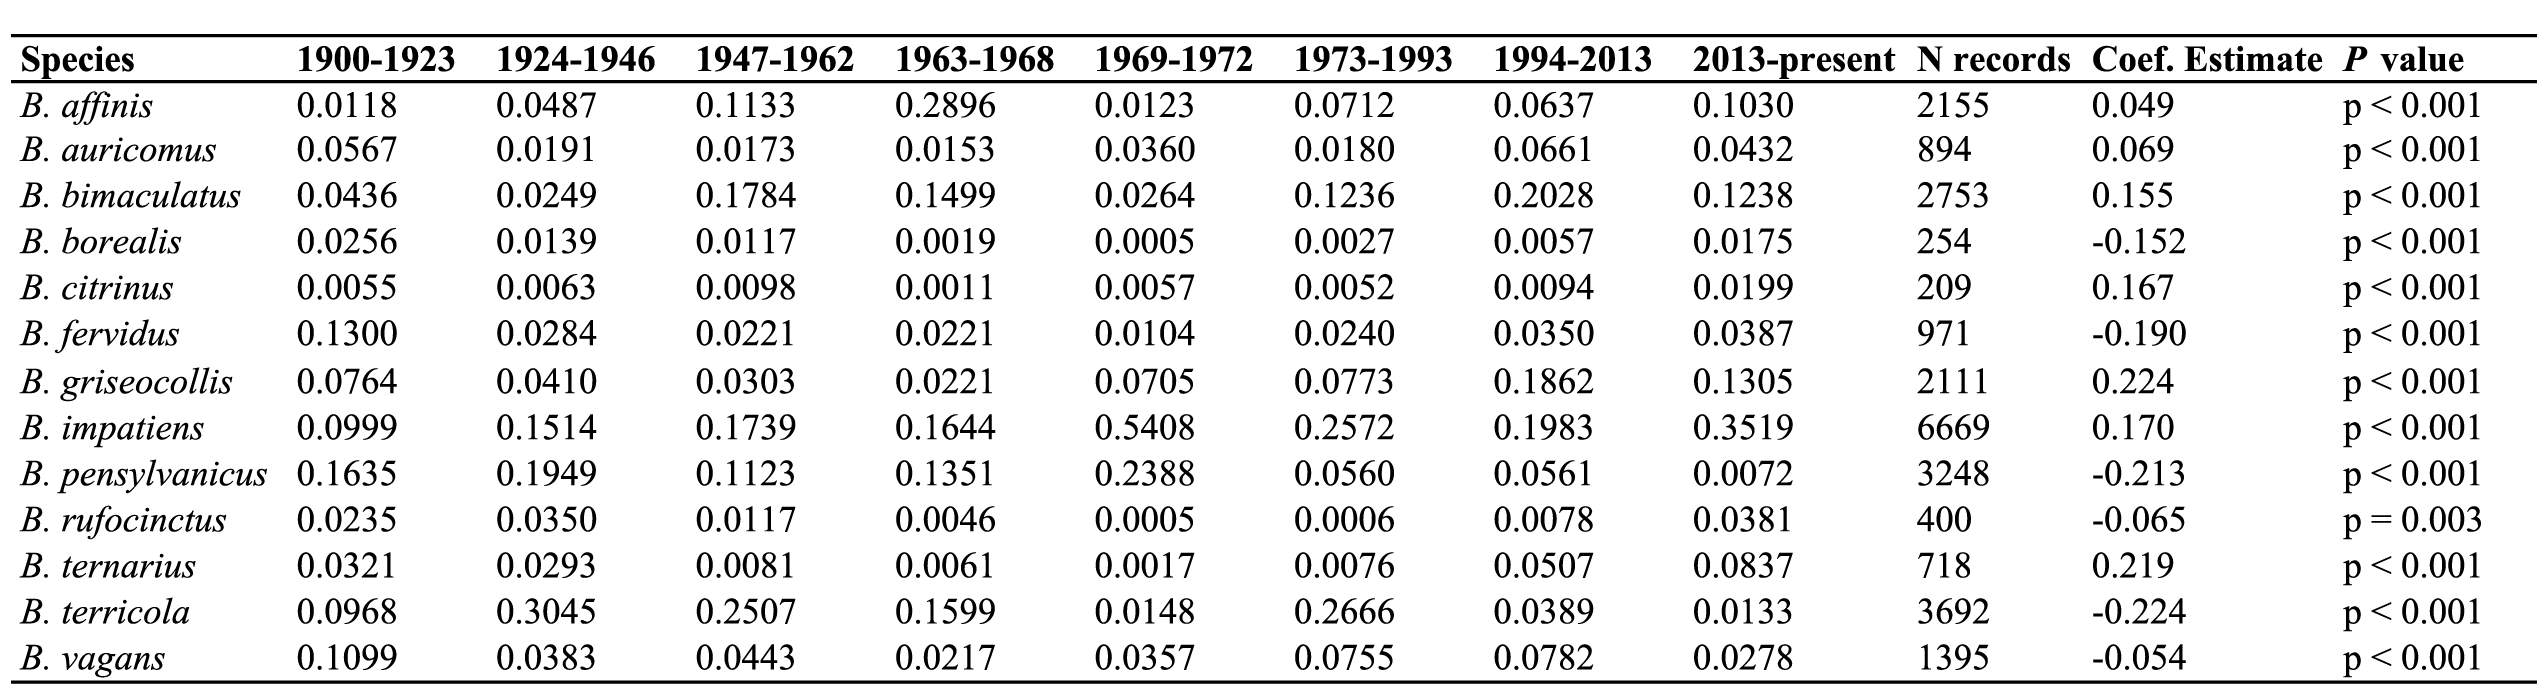
\includegraphics[width=1\textwidth,height=\textheight]{../ms_figs/table1.png}

\clearpage

\newpage

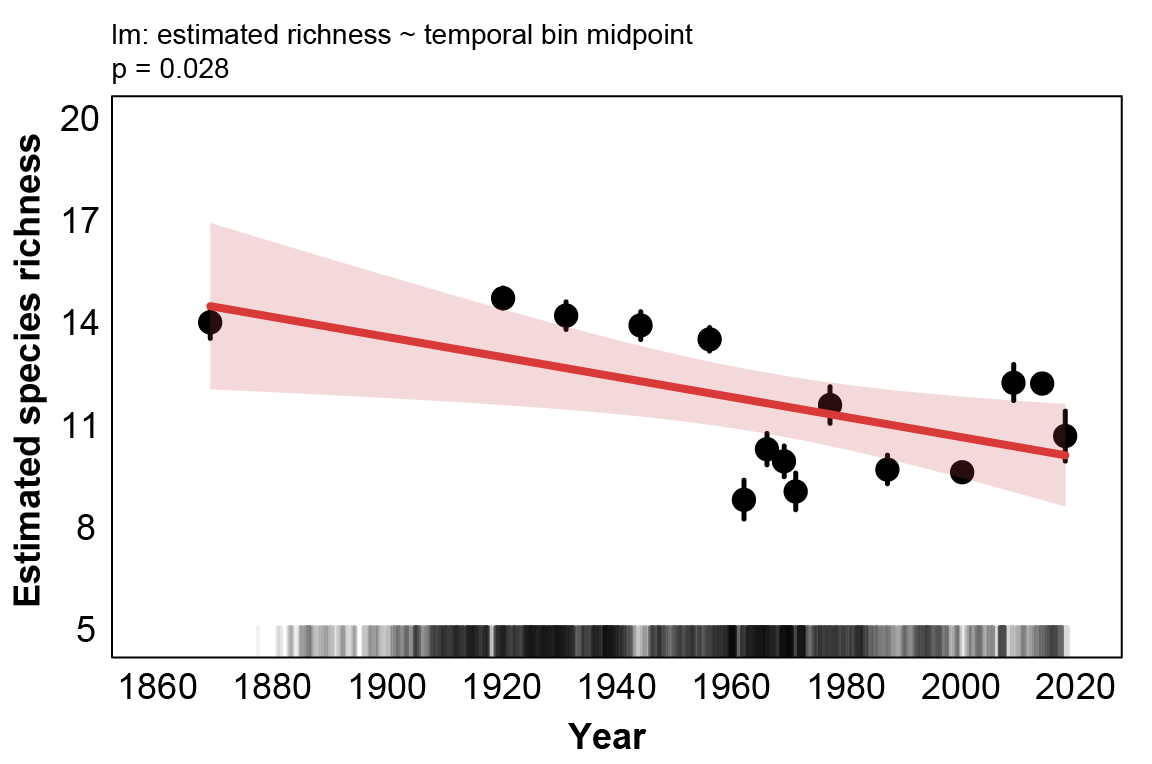
\includegraphics[width=0.6\textwidth,height=\textheight]{../ms_figs/fig1.png}

\textbf{Figure 1:} Trend in rarified bumble bee species richness from
1877-present. Each point represents a date range that is standardized to
contain an approximately equal number of bumble bee records. Each point
is plotted at the midpoint of the date range. The fitted line is a
linear model predicting estimated species richness as a function of
temporal bin order using the midpoint of the temporal bin as the
predictor. Carpet plot represents temporal collection point for all
records from 1877 to present.

\clearpage

\newpage

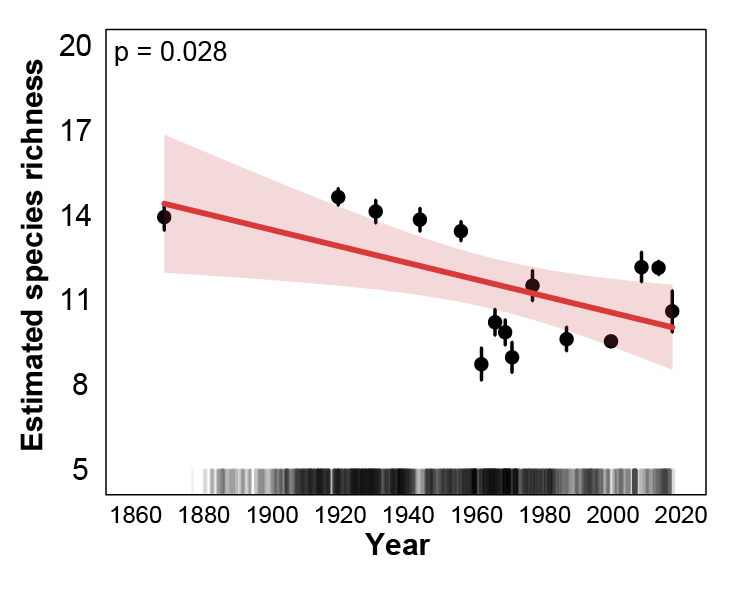
\includegraphics[width=1\textwidth,height=\textheight]{../ms_figs/fig2.png}

\textbf{Figure 2:} Patterns of agricultural intensification in two
metrics: (a) proportion of county under cultivation and (c) number of
crops grown per county. Inset graphs (b,d) depict general trend of these
variables for each state in the study area as modeled by a Loess fitted
curve. Values beneath years are mean ± SEM.

\clearpage

\newpage

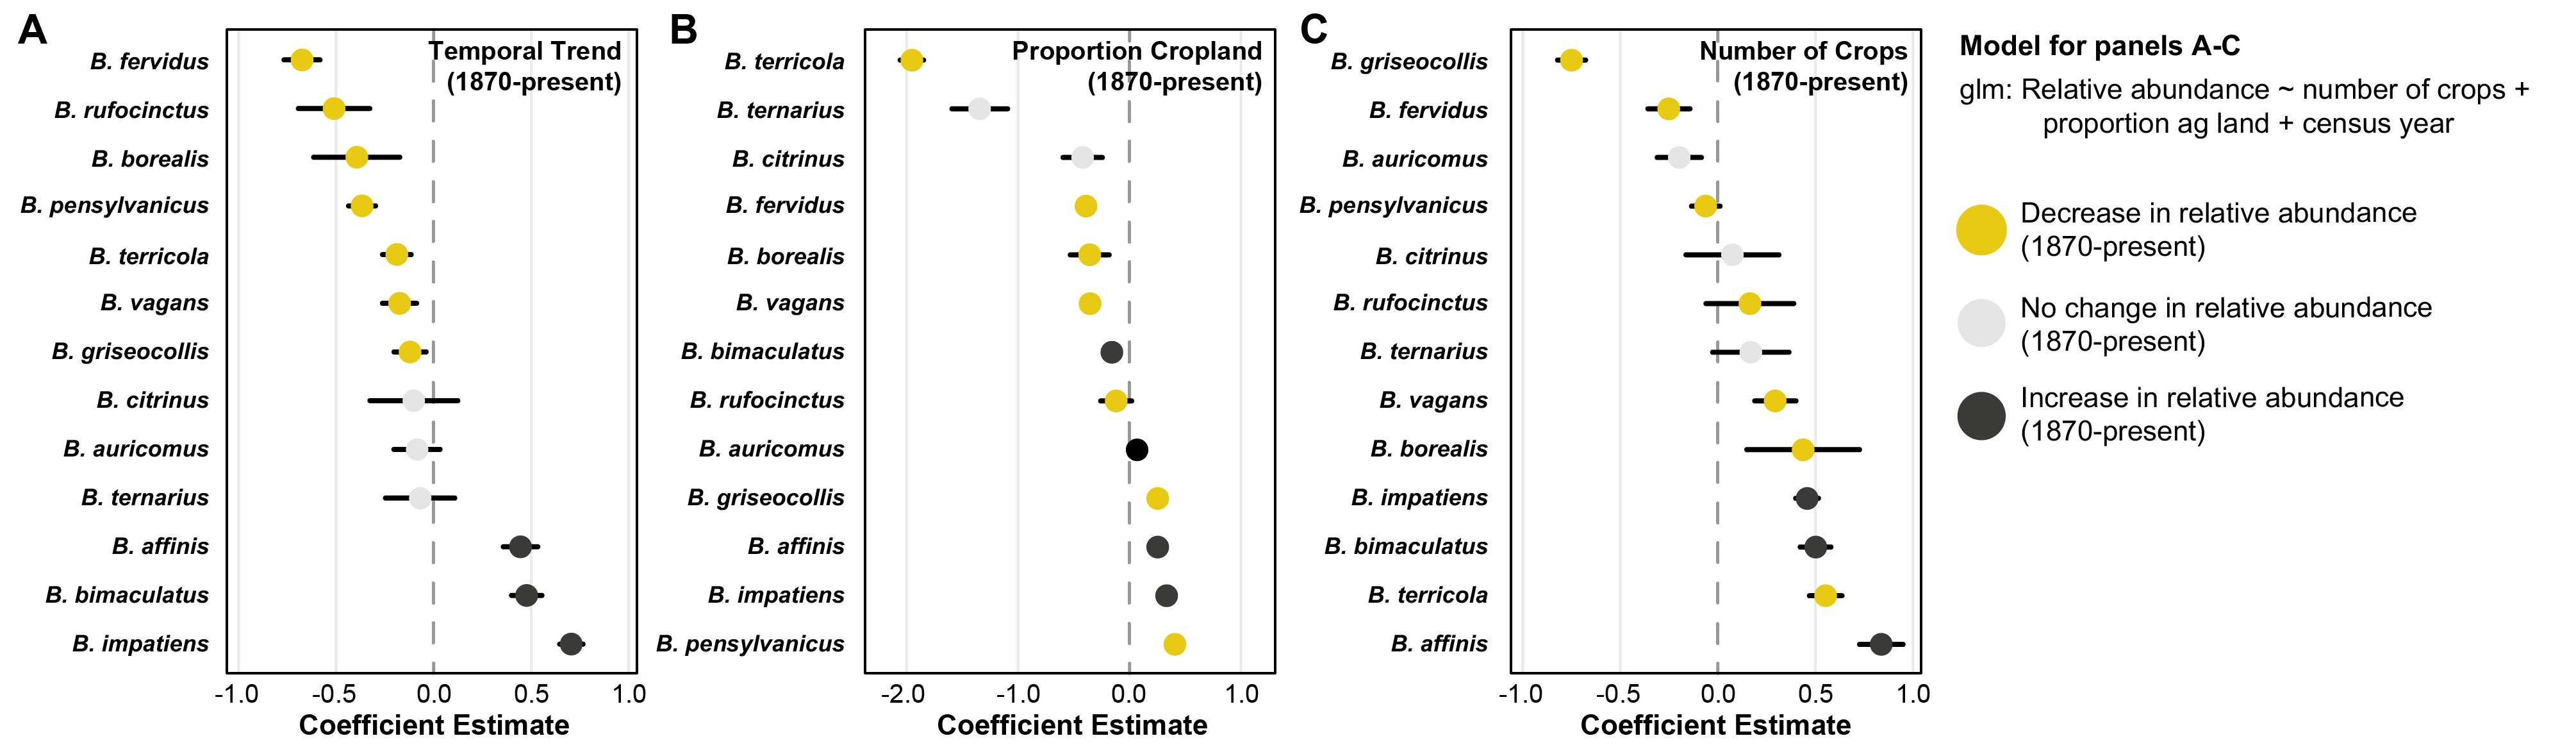
\includegraphics[width=1\textwidth,height=\textheight]{../ms_figs/fig3.png}

\textbf{Figure 3:} Fitted model coefficients (± 95\% confidence
interval) for each study species for (A) temporal trend of the species,
(B) proportion of county in cropland, and (C) the number of crops grown
in a county. Models were fitted using the entire dataset from
1870-present. Point colors indicate species relative abundance trend
from 1870-present: yellow points denote species whose relative abundance
declined, gray points denote no change in relative abundance, and black
points denote increases in relative abundance.

\clearpage

\newpage

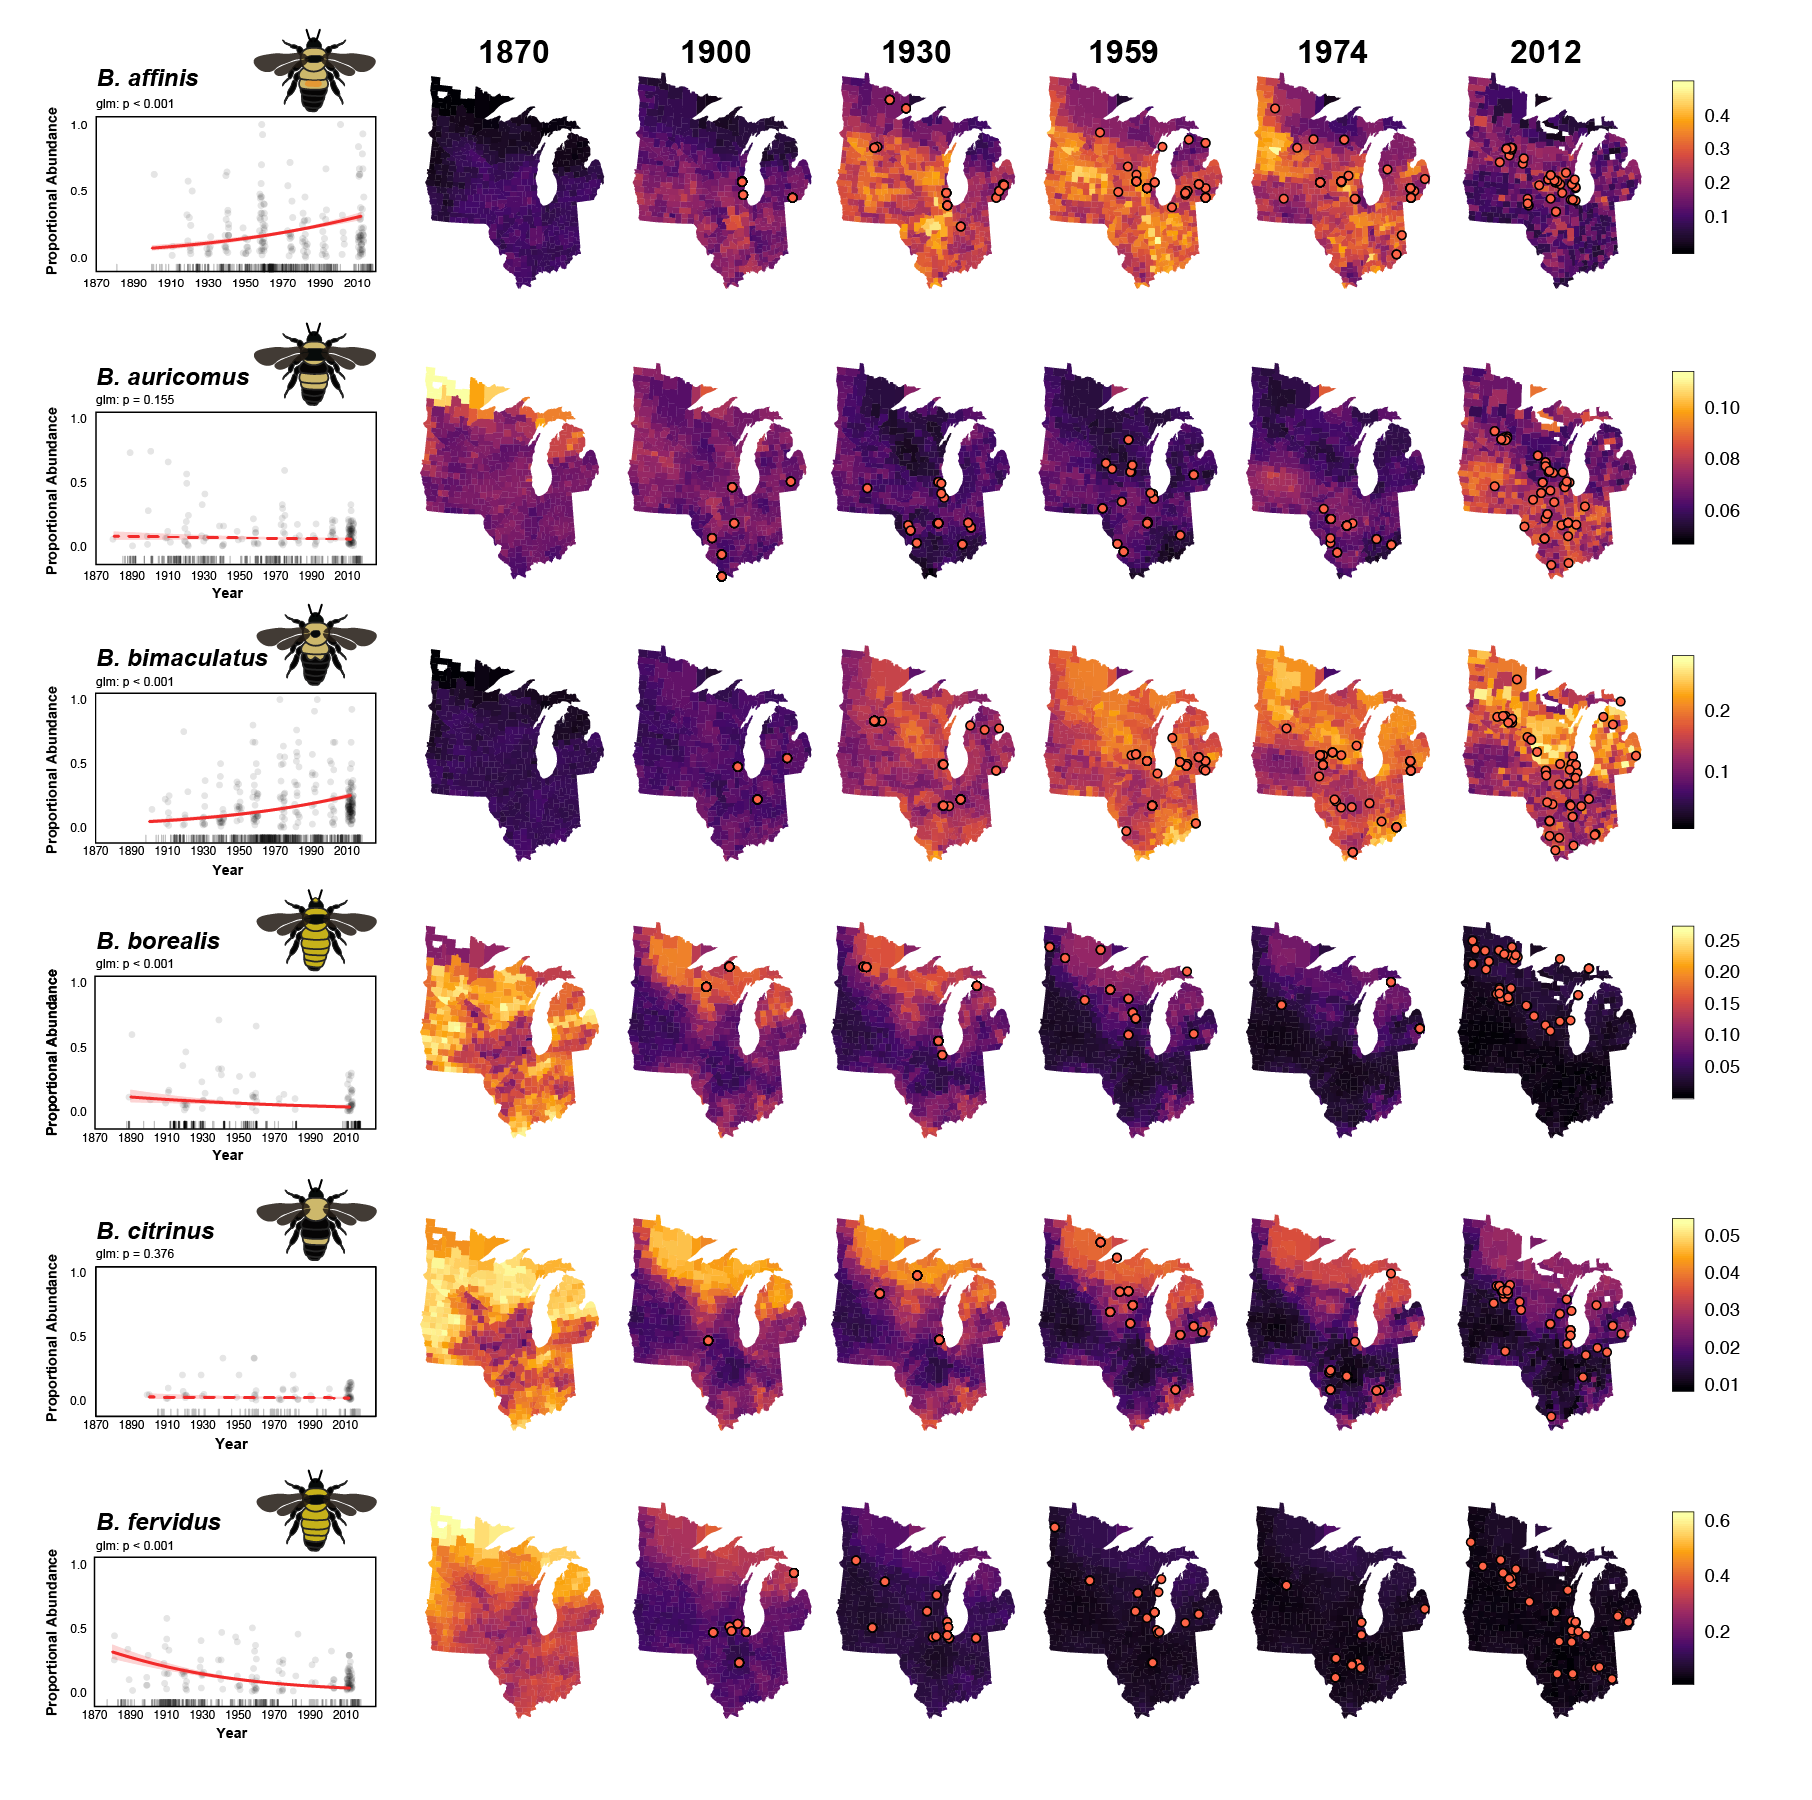
\includegraphics[width=1\textwidth,height=\textheight]{../ms_figs/fig4a.png}

\clearpage

\newpage

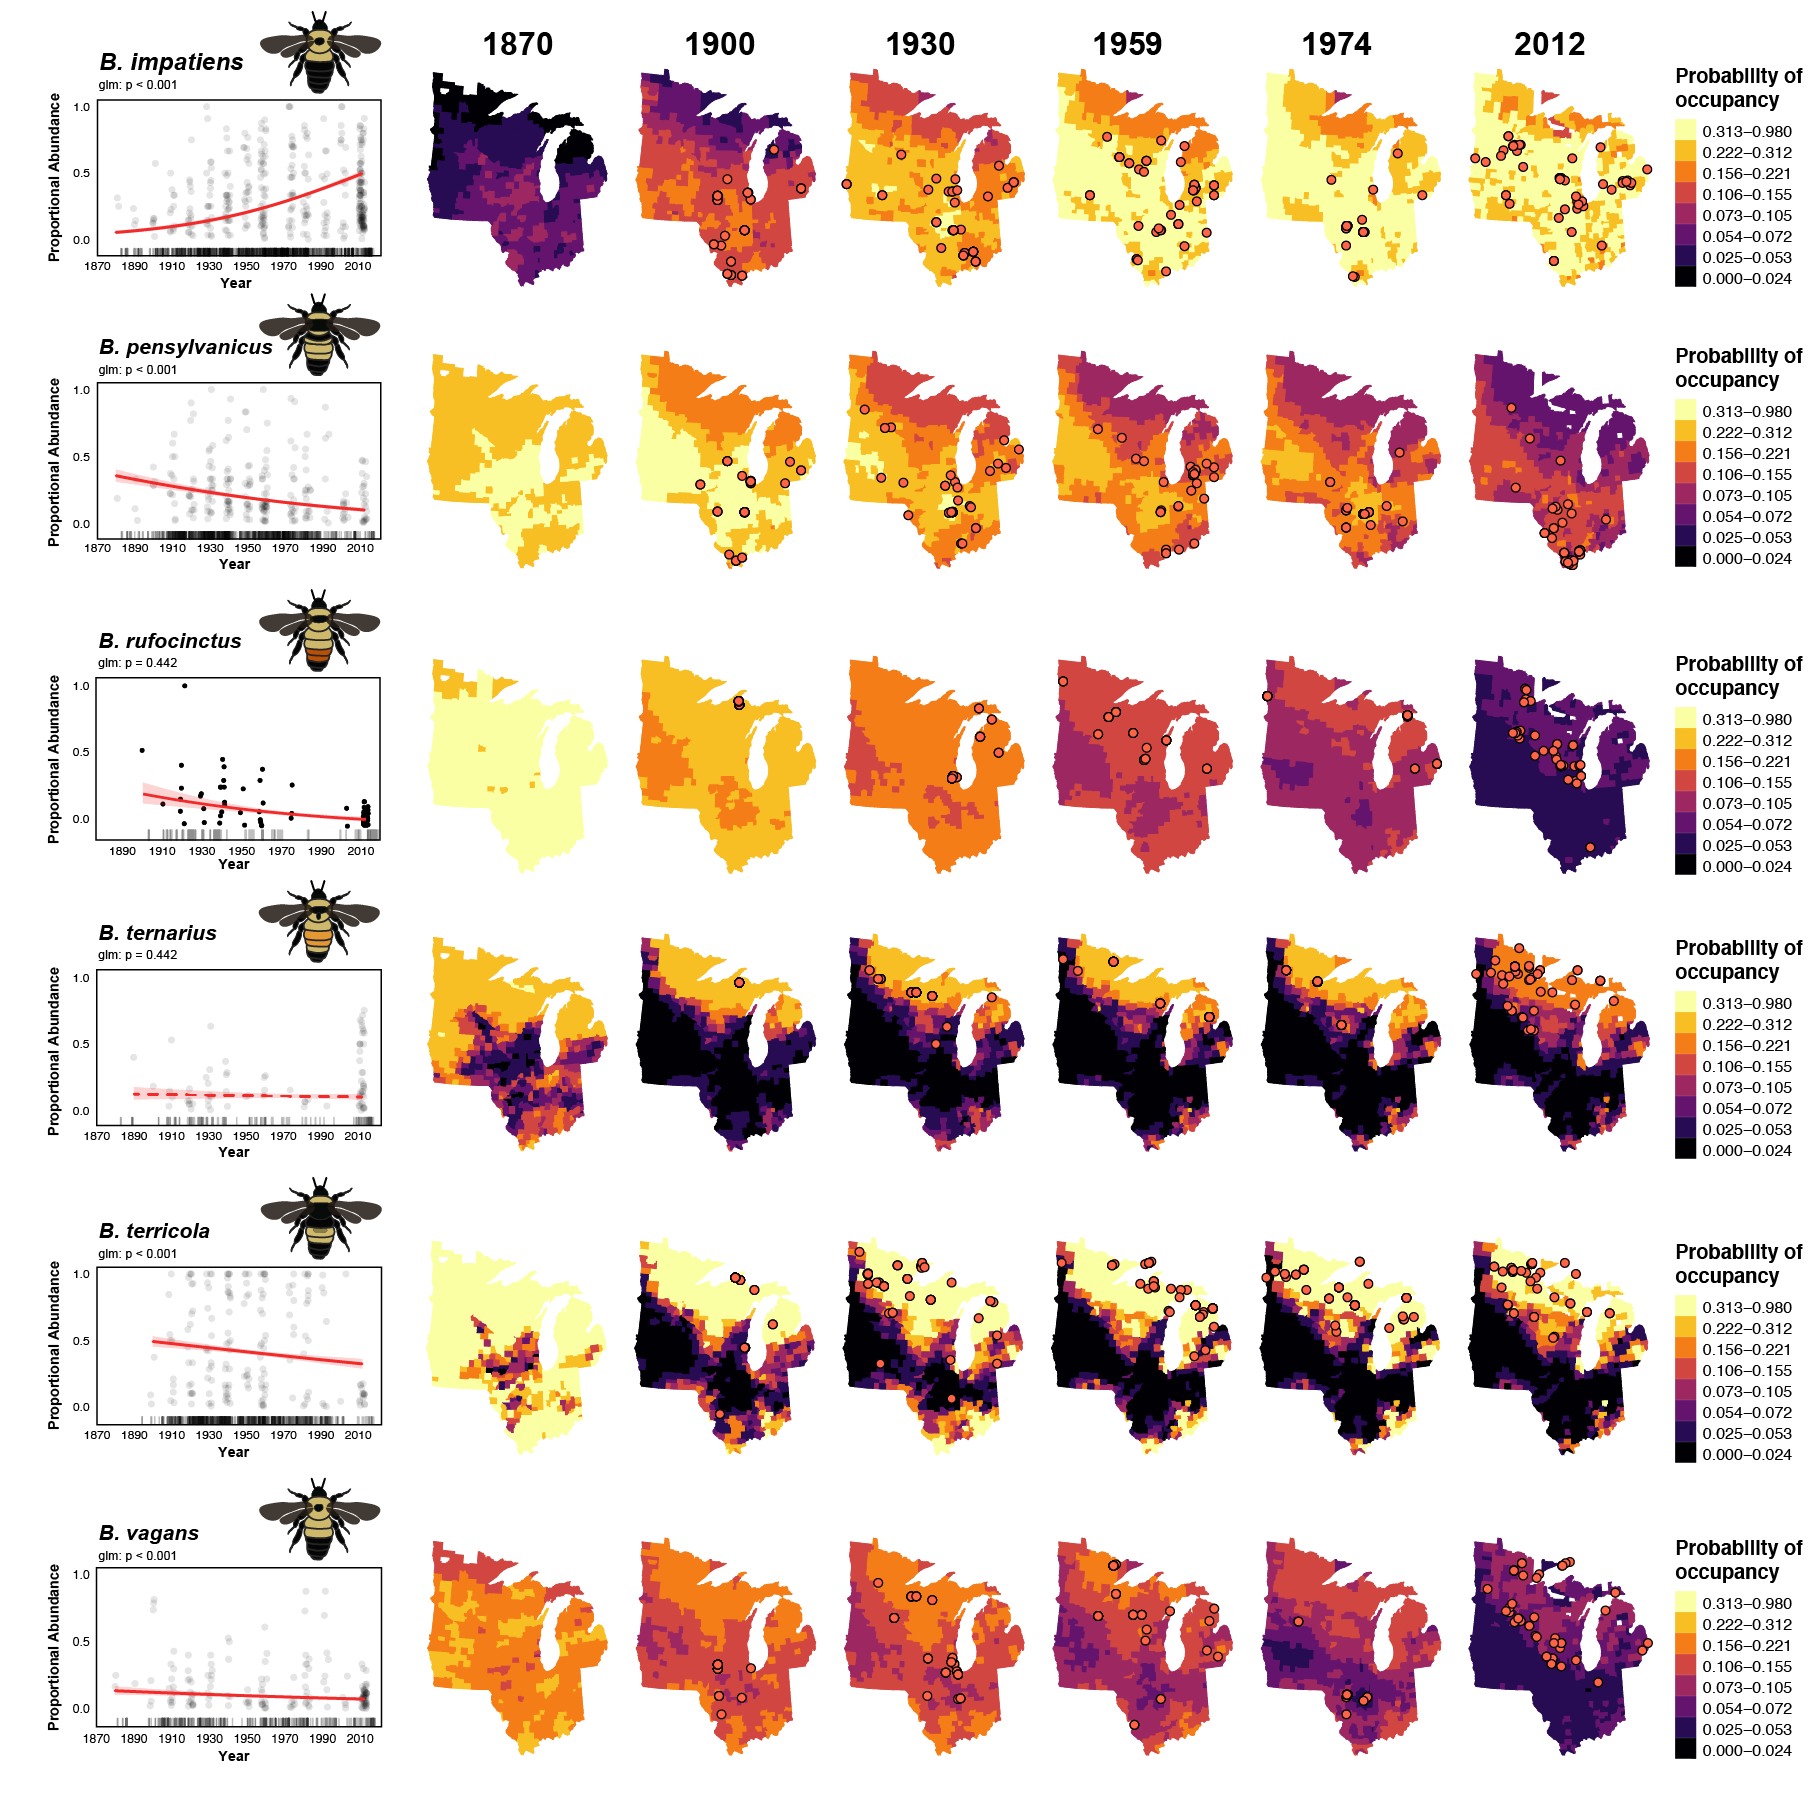
\includegraphics[width=1\textwidth,height=\textheight]{../ms_figs/fig4b.png}

\textbf{Figure 4:} Fitted temporal trend of relative abundance when
modeled with agricultural intensity metrics along with the predicted
probability of occurrence for each study species in each county given
crop diversity and proportion cropland in each county. Darker colors
denote smaller probability of occurrence, while lighter colors indicate
larger probability of occurrence. Solid red lines denote statistically
clear trend in relative abundance over time (p \textless{} 0.05), while
dashed lines denote statistically unclear trends (p \textgreater{}
0.05). Points on temporal trend are slightly jittered for visibility.
Red points on each map are randomly selected occurrence records with a
maximum of 50 plotted per year.

\clearpage

\newpage

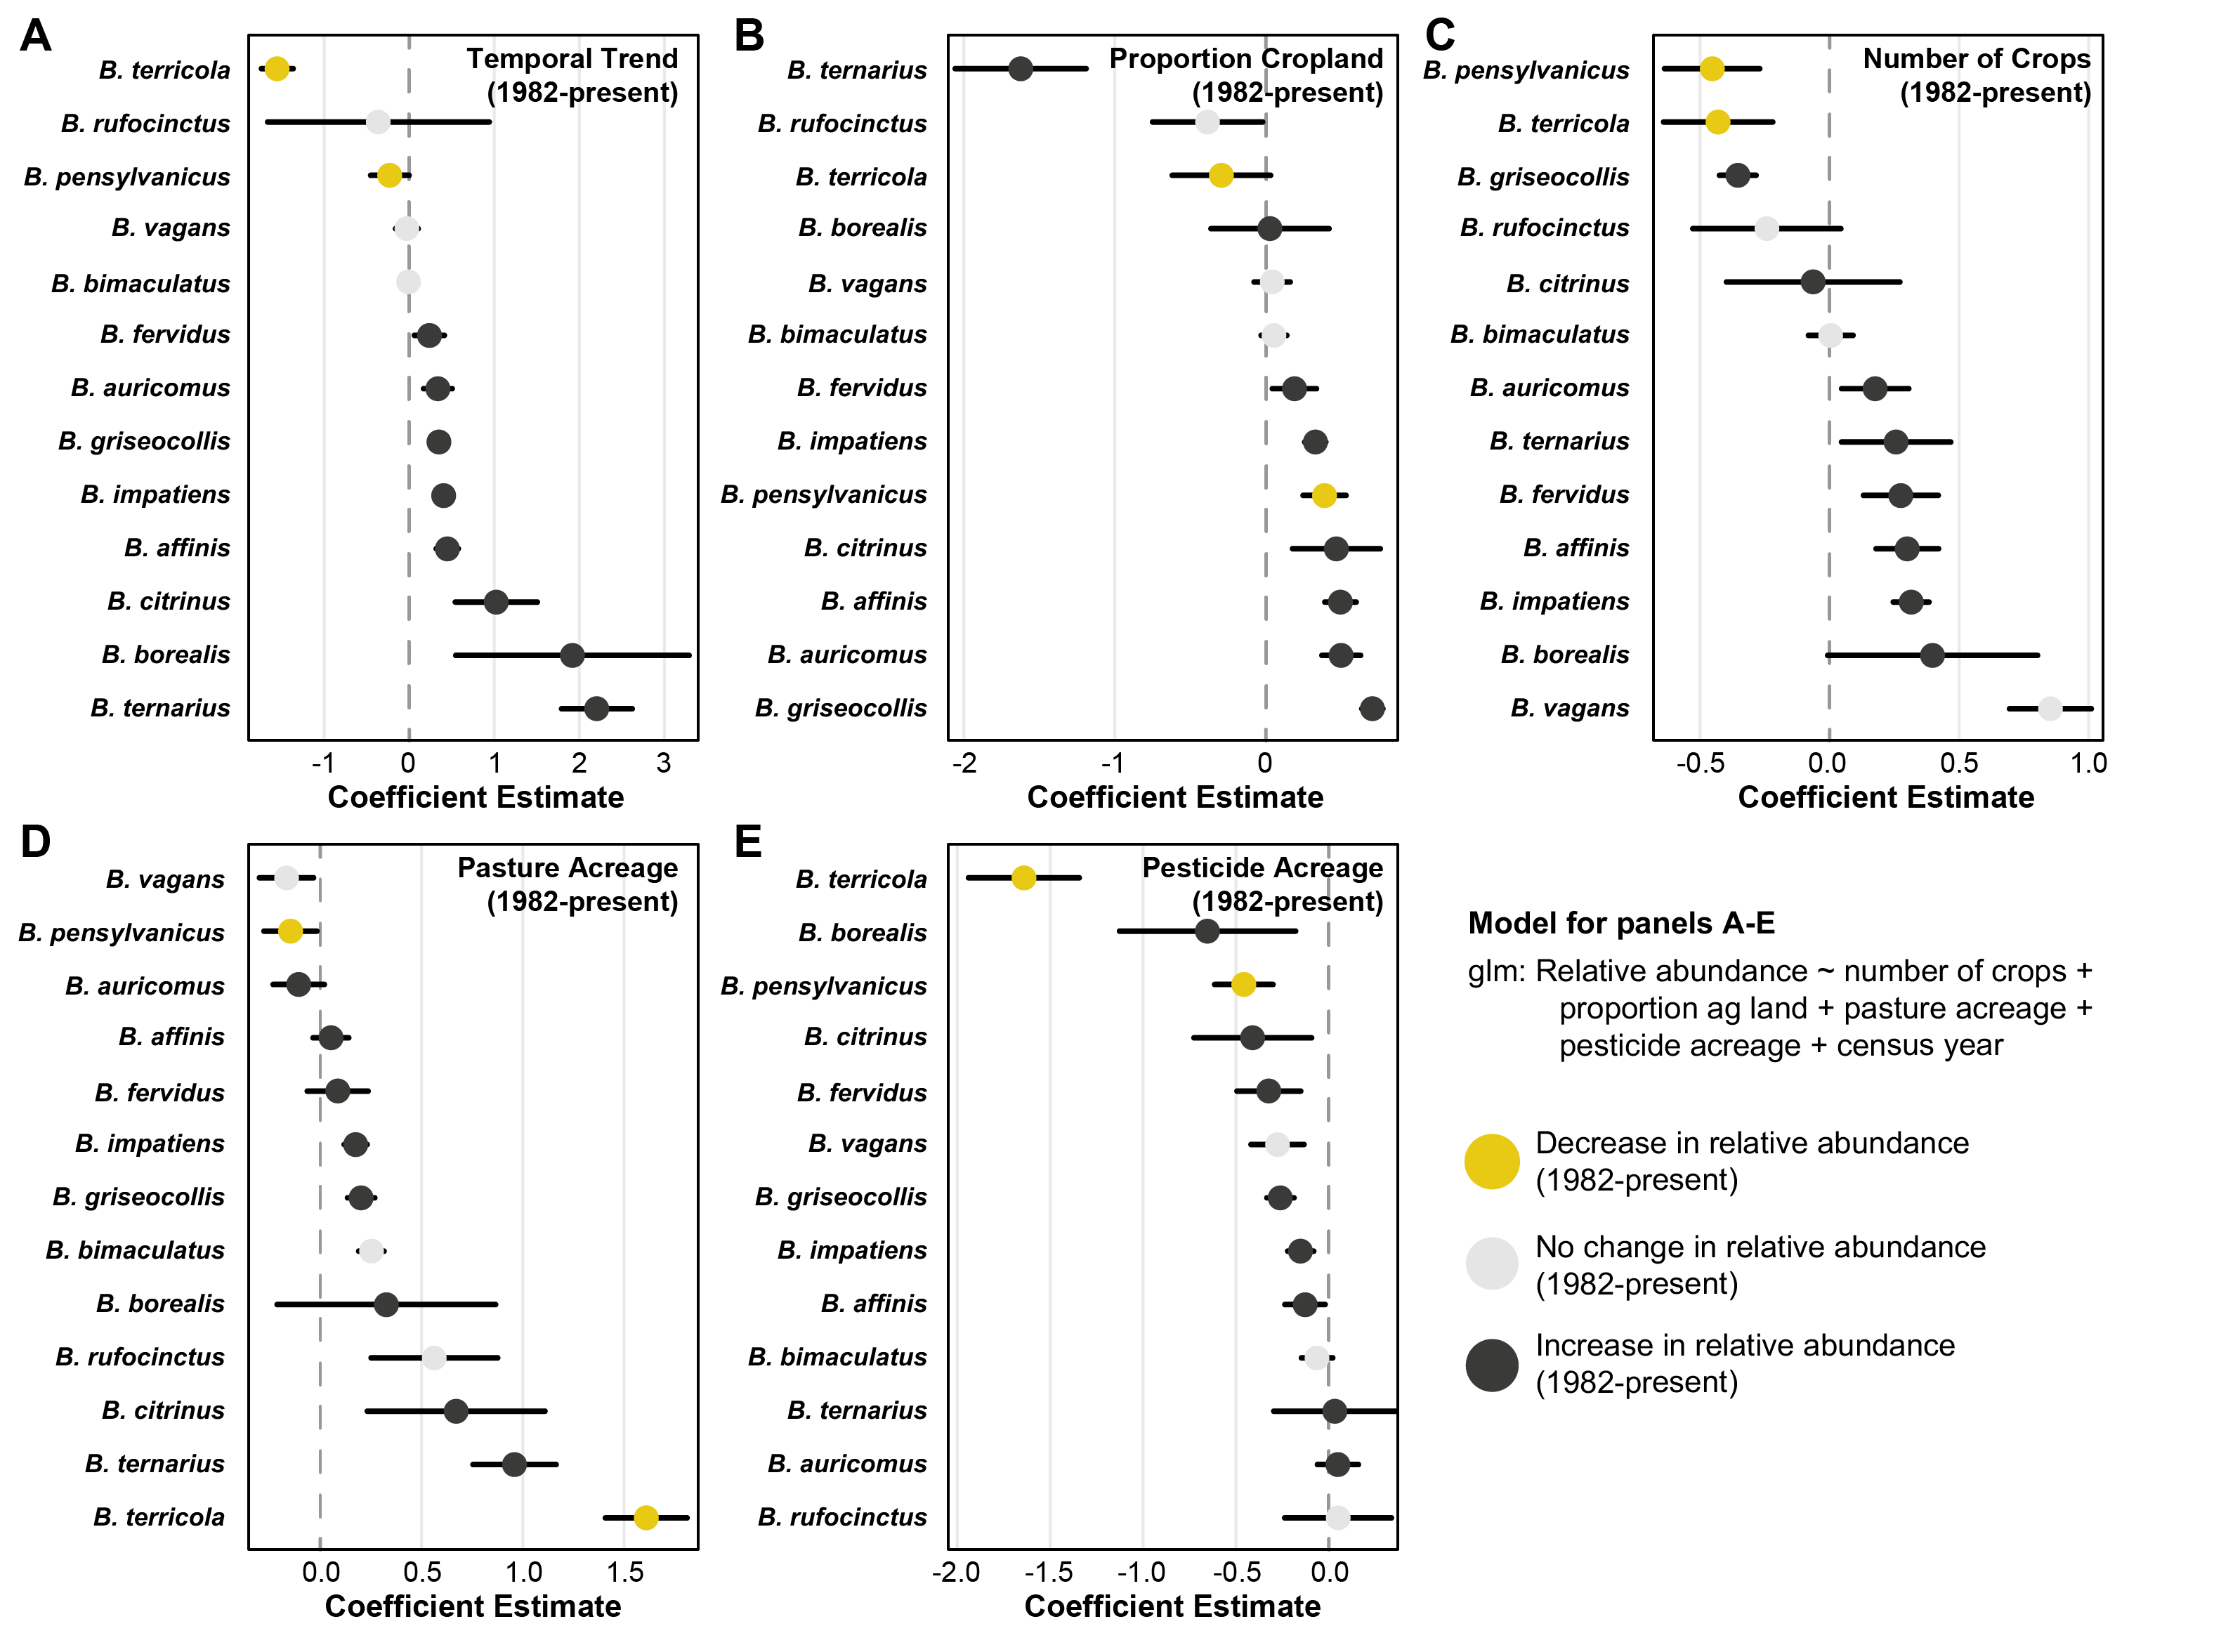
\includegraphics[width=1\textwidth,height=\textheight]{../ms_figs/fig4.png}

\textbf{Figure 5:} Fitted model coefficients (± 95\% confidence
interval) for each study species for (A) temporal trend of the species,
(B) proportion of county in cropland, and (C) the number of crops grown
in a county, (D) acres of pasture grown in a county, and (E) acres
treated with insecticides. Models were fitted using data from
1982-present (only years for which pesticide and pasture acreage are
available across all counties). Point colors indicate species relative
abundance trend from 1982-present: yellow points denote species whose
relative abundance declined, gray points denote no change in relative
abundance, and black points denote increases in relative abundance.

\clearpage

\newpage

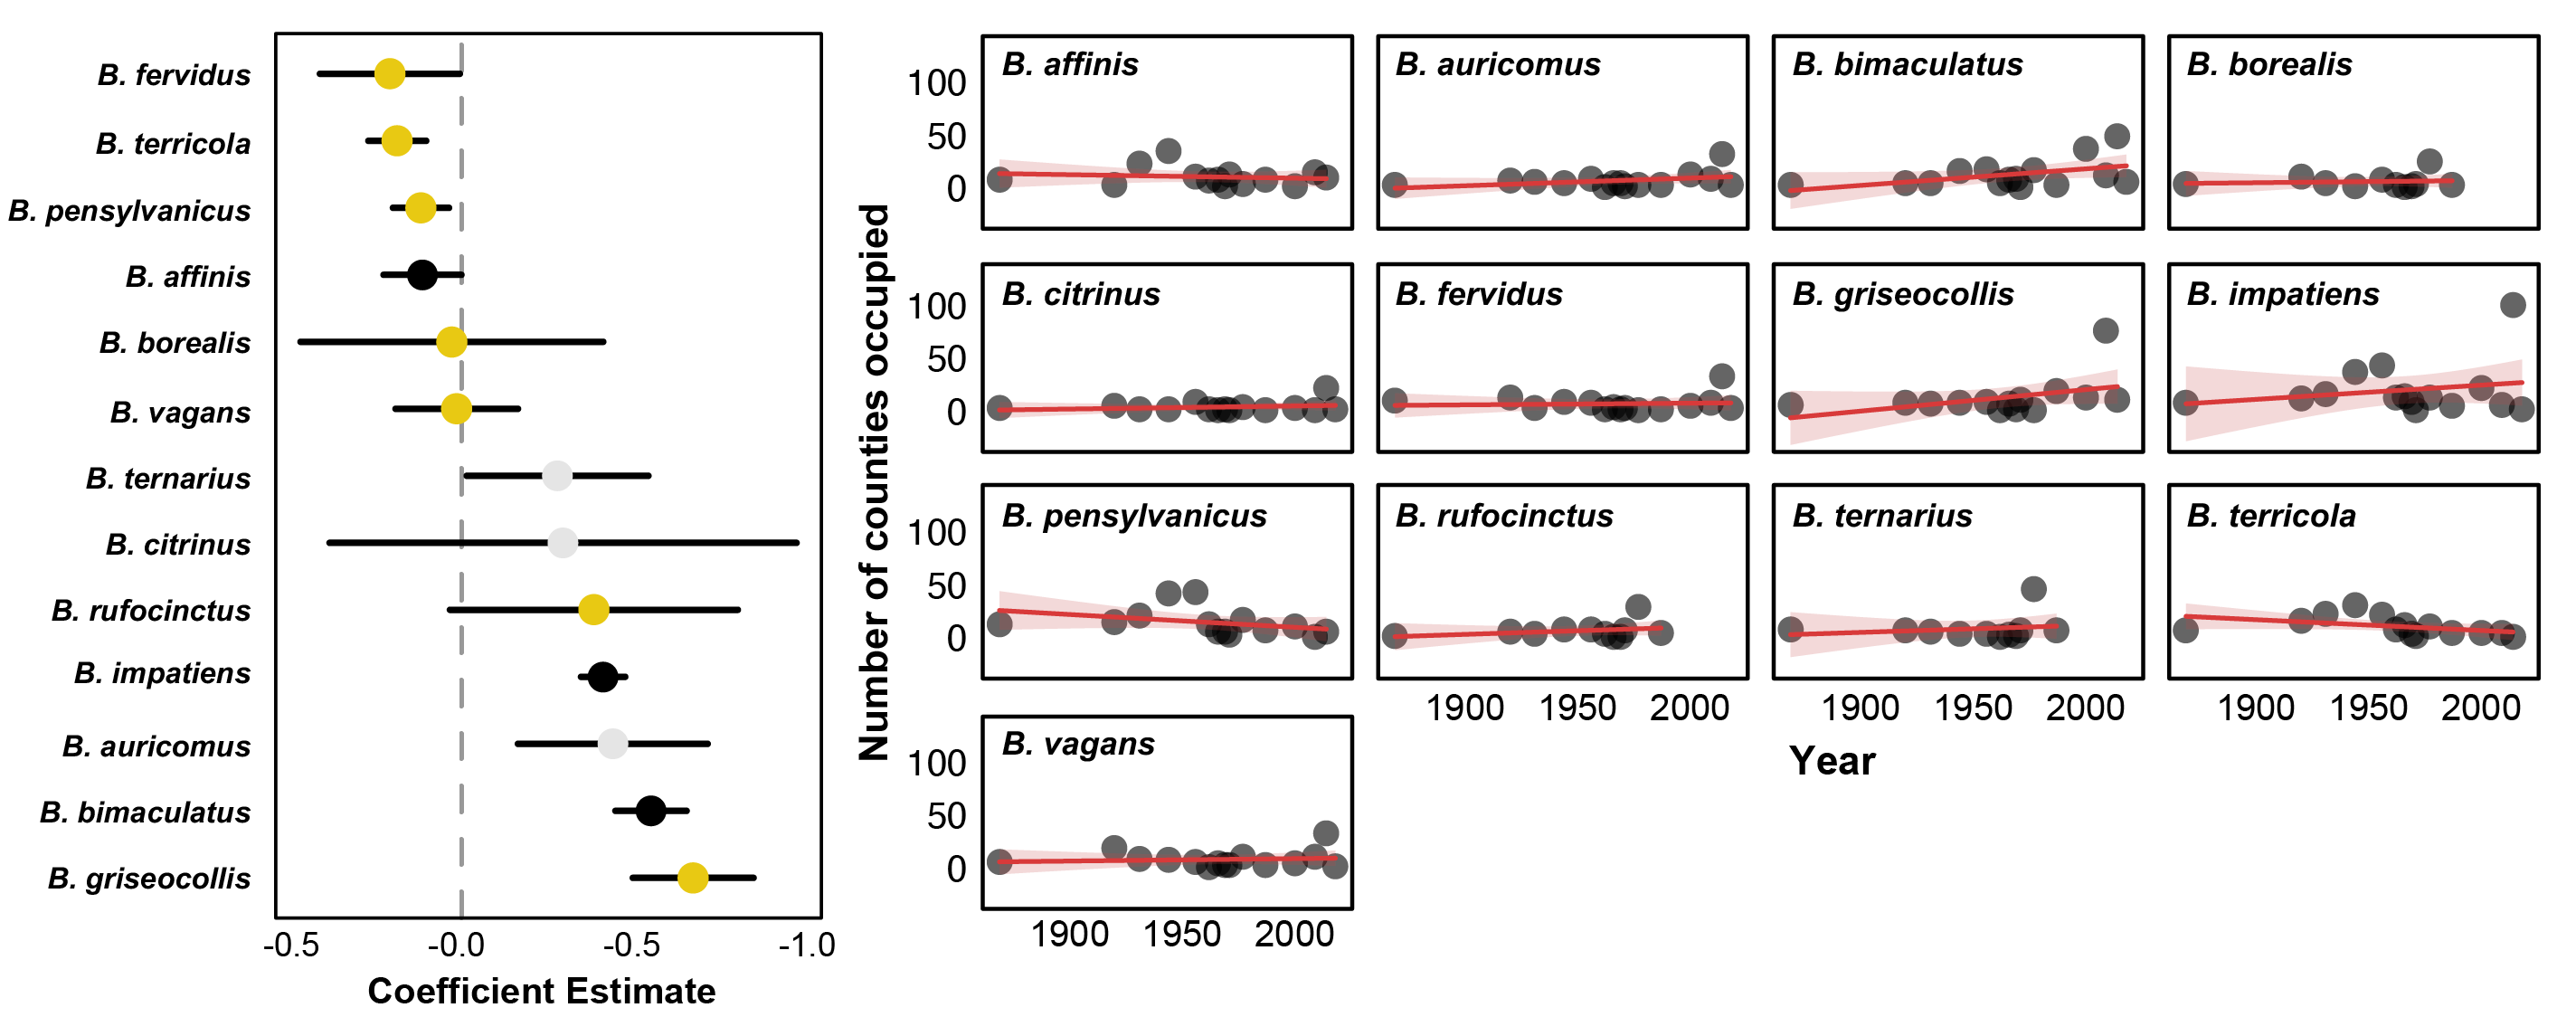
\includegraphics[width=1\textwidth,height=\textheight]{../ms_figs/fig6.png}

\textbf{Figure 6:} (A) Fitted model coefficients for each species for
change in county occupancy over time. (B) For each species, plotted
temporal trends of county occupancy over time with fitted GLM models
with 95\% confidence interval. Point colors indicate species relative
abundance trend from 1870-present: red points denote species whose
relative abundance declined, black points denote no change in relative
abundance, and blue points denote increases in relative abundance.

\clearpage

\newpage

\hypertarget{supplementary-material}{%
\section{Supplementary Material}\label{supplementary-material}}

\textbf{Supplementary Table 1:} Generalized linear model results for
each study species including the sample size (number of counties for
which relative abundance is calculated), model term, scaled coefficient
estimate, 95\% confidence interval and p-value. Each county is weighted
by the total number of bumble bee records for a given time point
(agricultural census year).

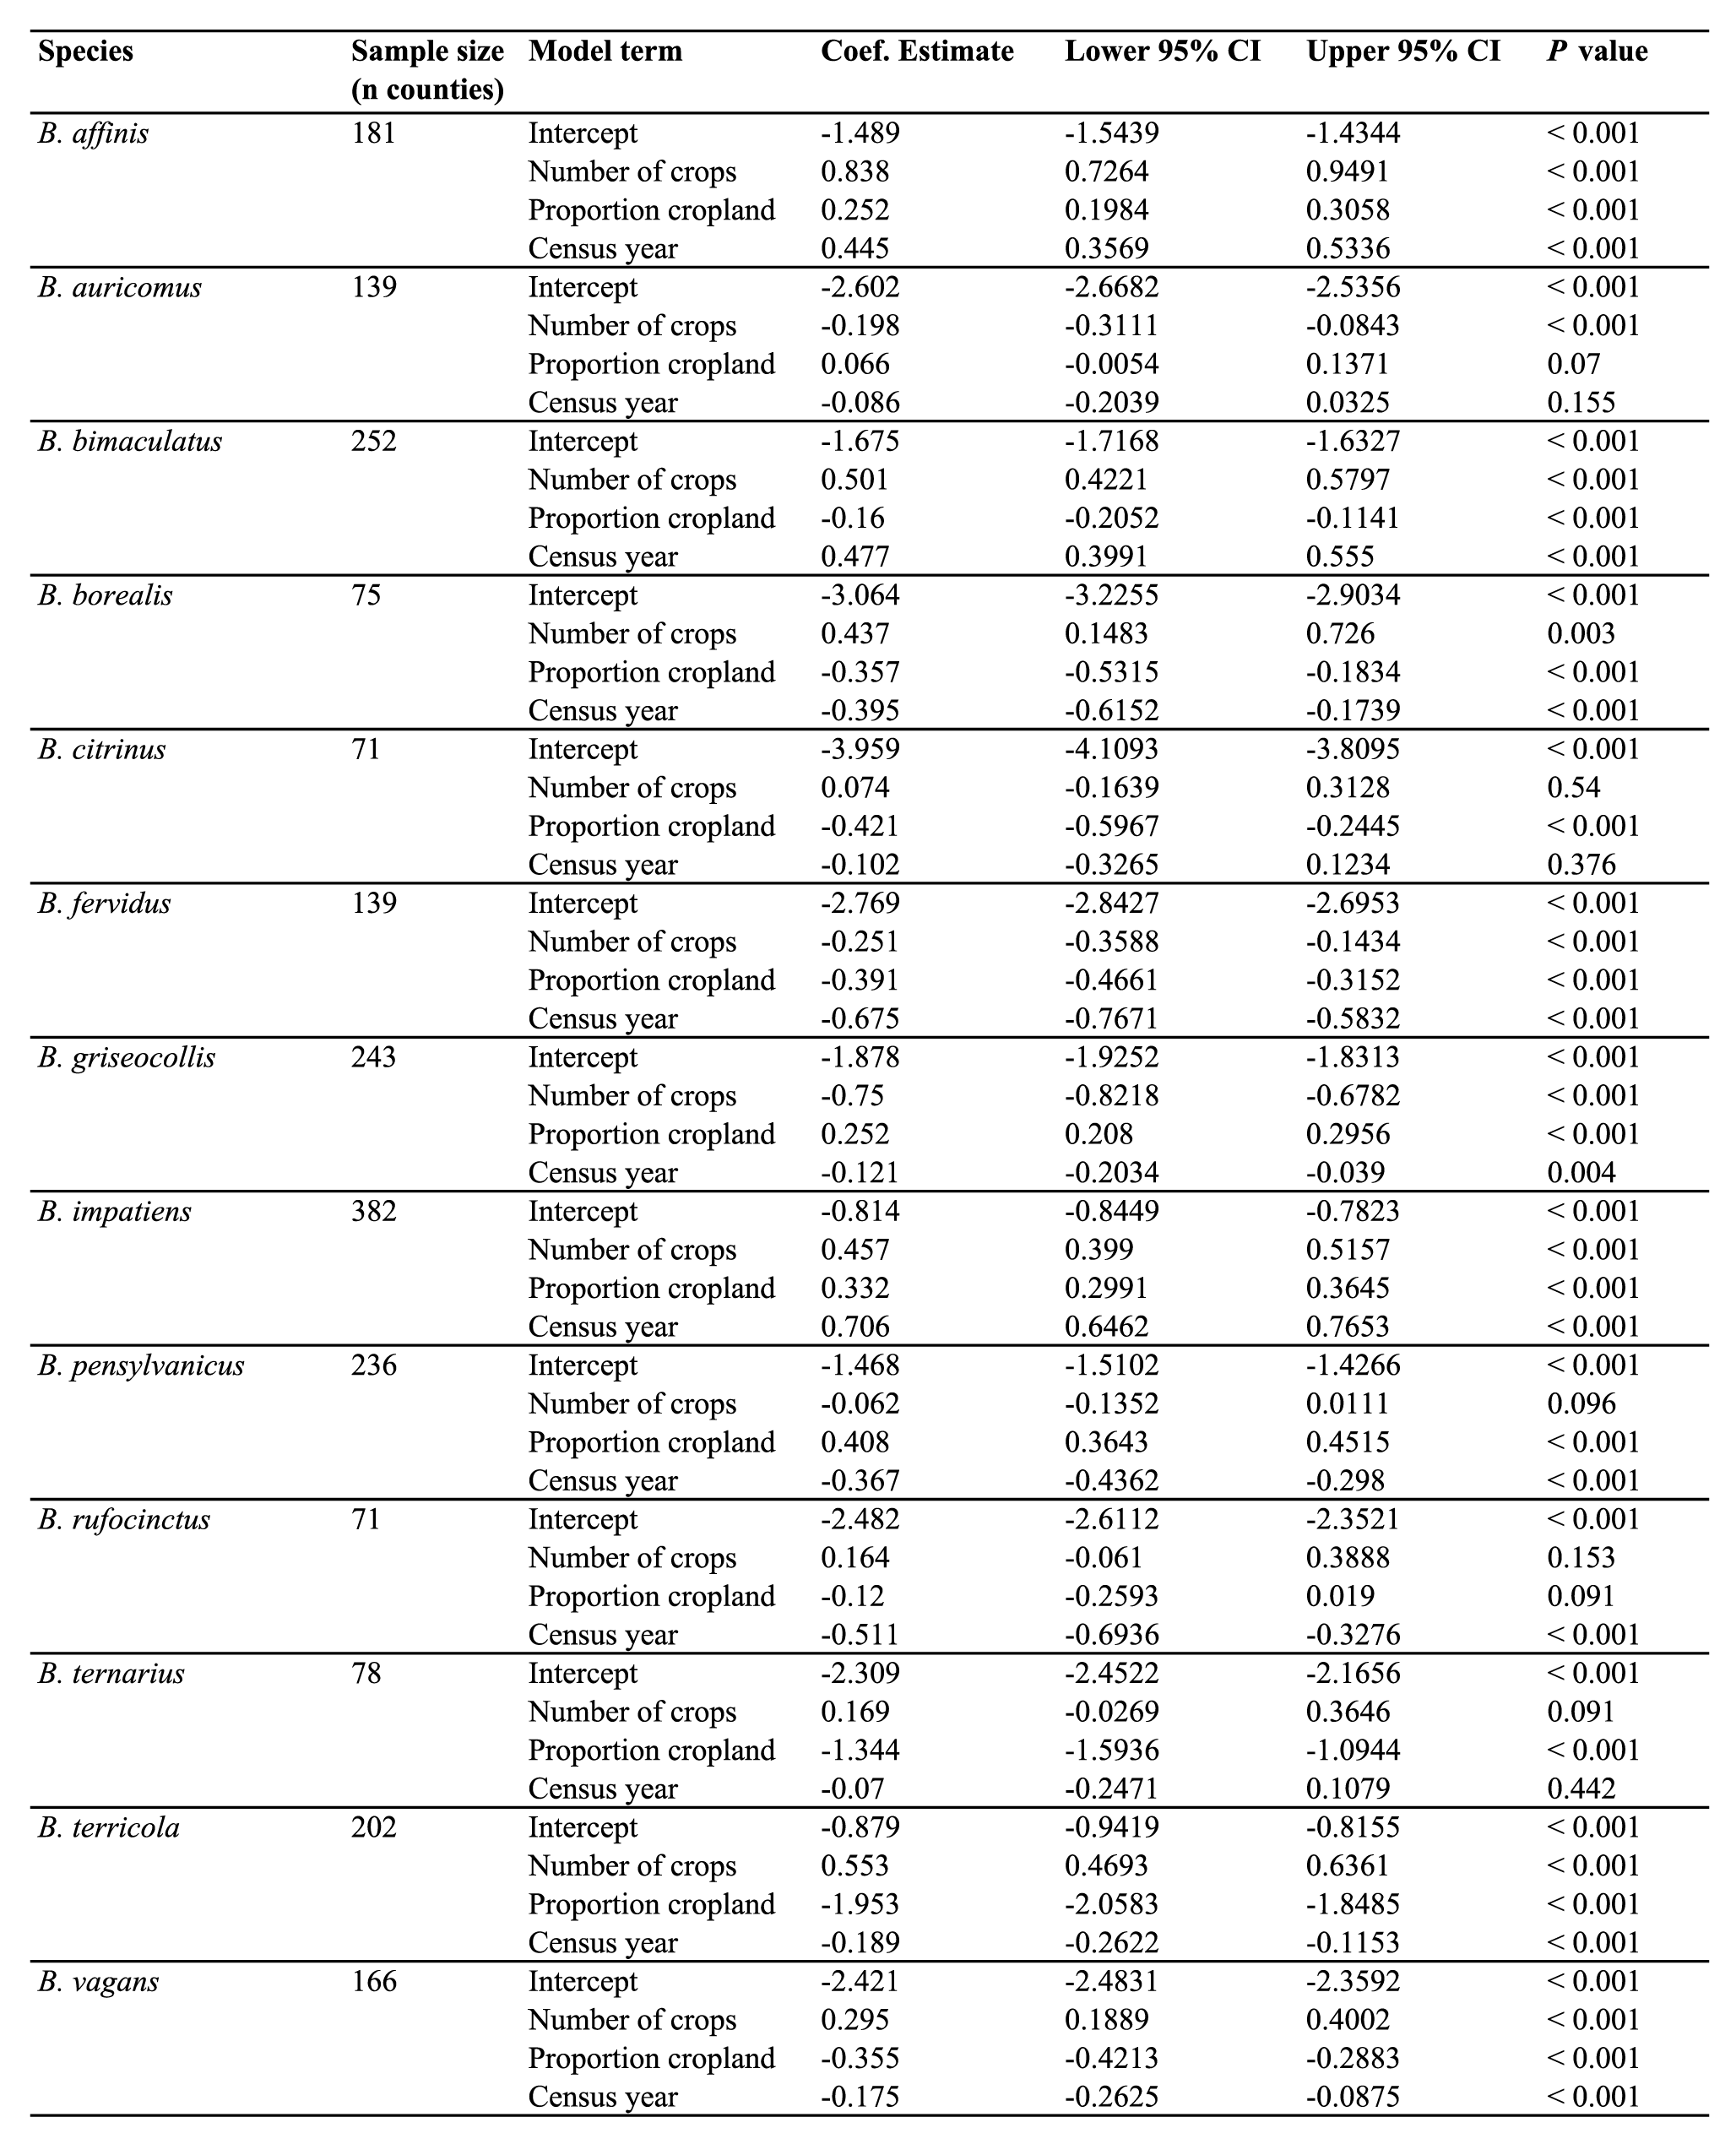
\includegraphics[width=0.6\textwidth,height=\textheight]{../ms_figs/tables1.png}

\clearpage

\newpage

\textbf{Supplementary Table 2:} Generalized linear model results for
each study species including the sample size (number of counties for
which relative abundance is calculated), model term, scaled coefficient
estimate, 95\% confidence interval and p-value. Each county is weighted
by the total number of bumble bee records for a given time point
(agricultural census year).

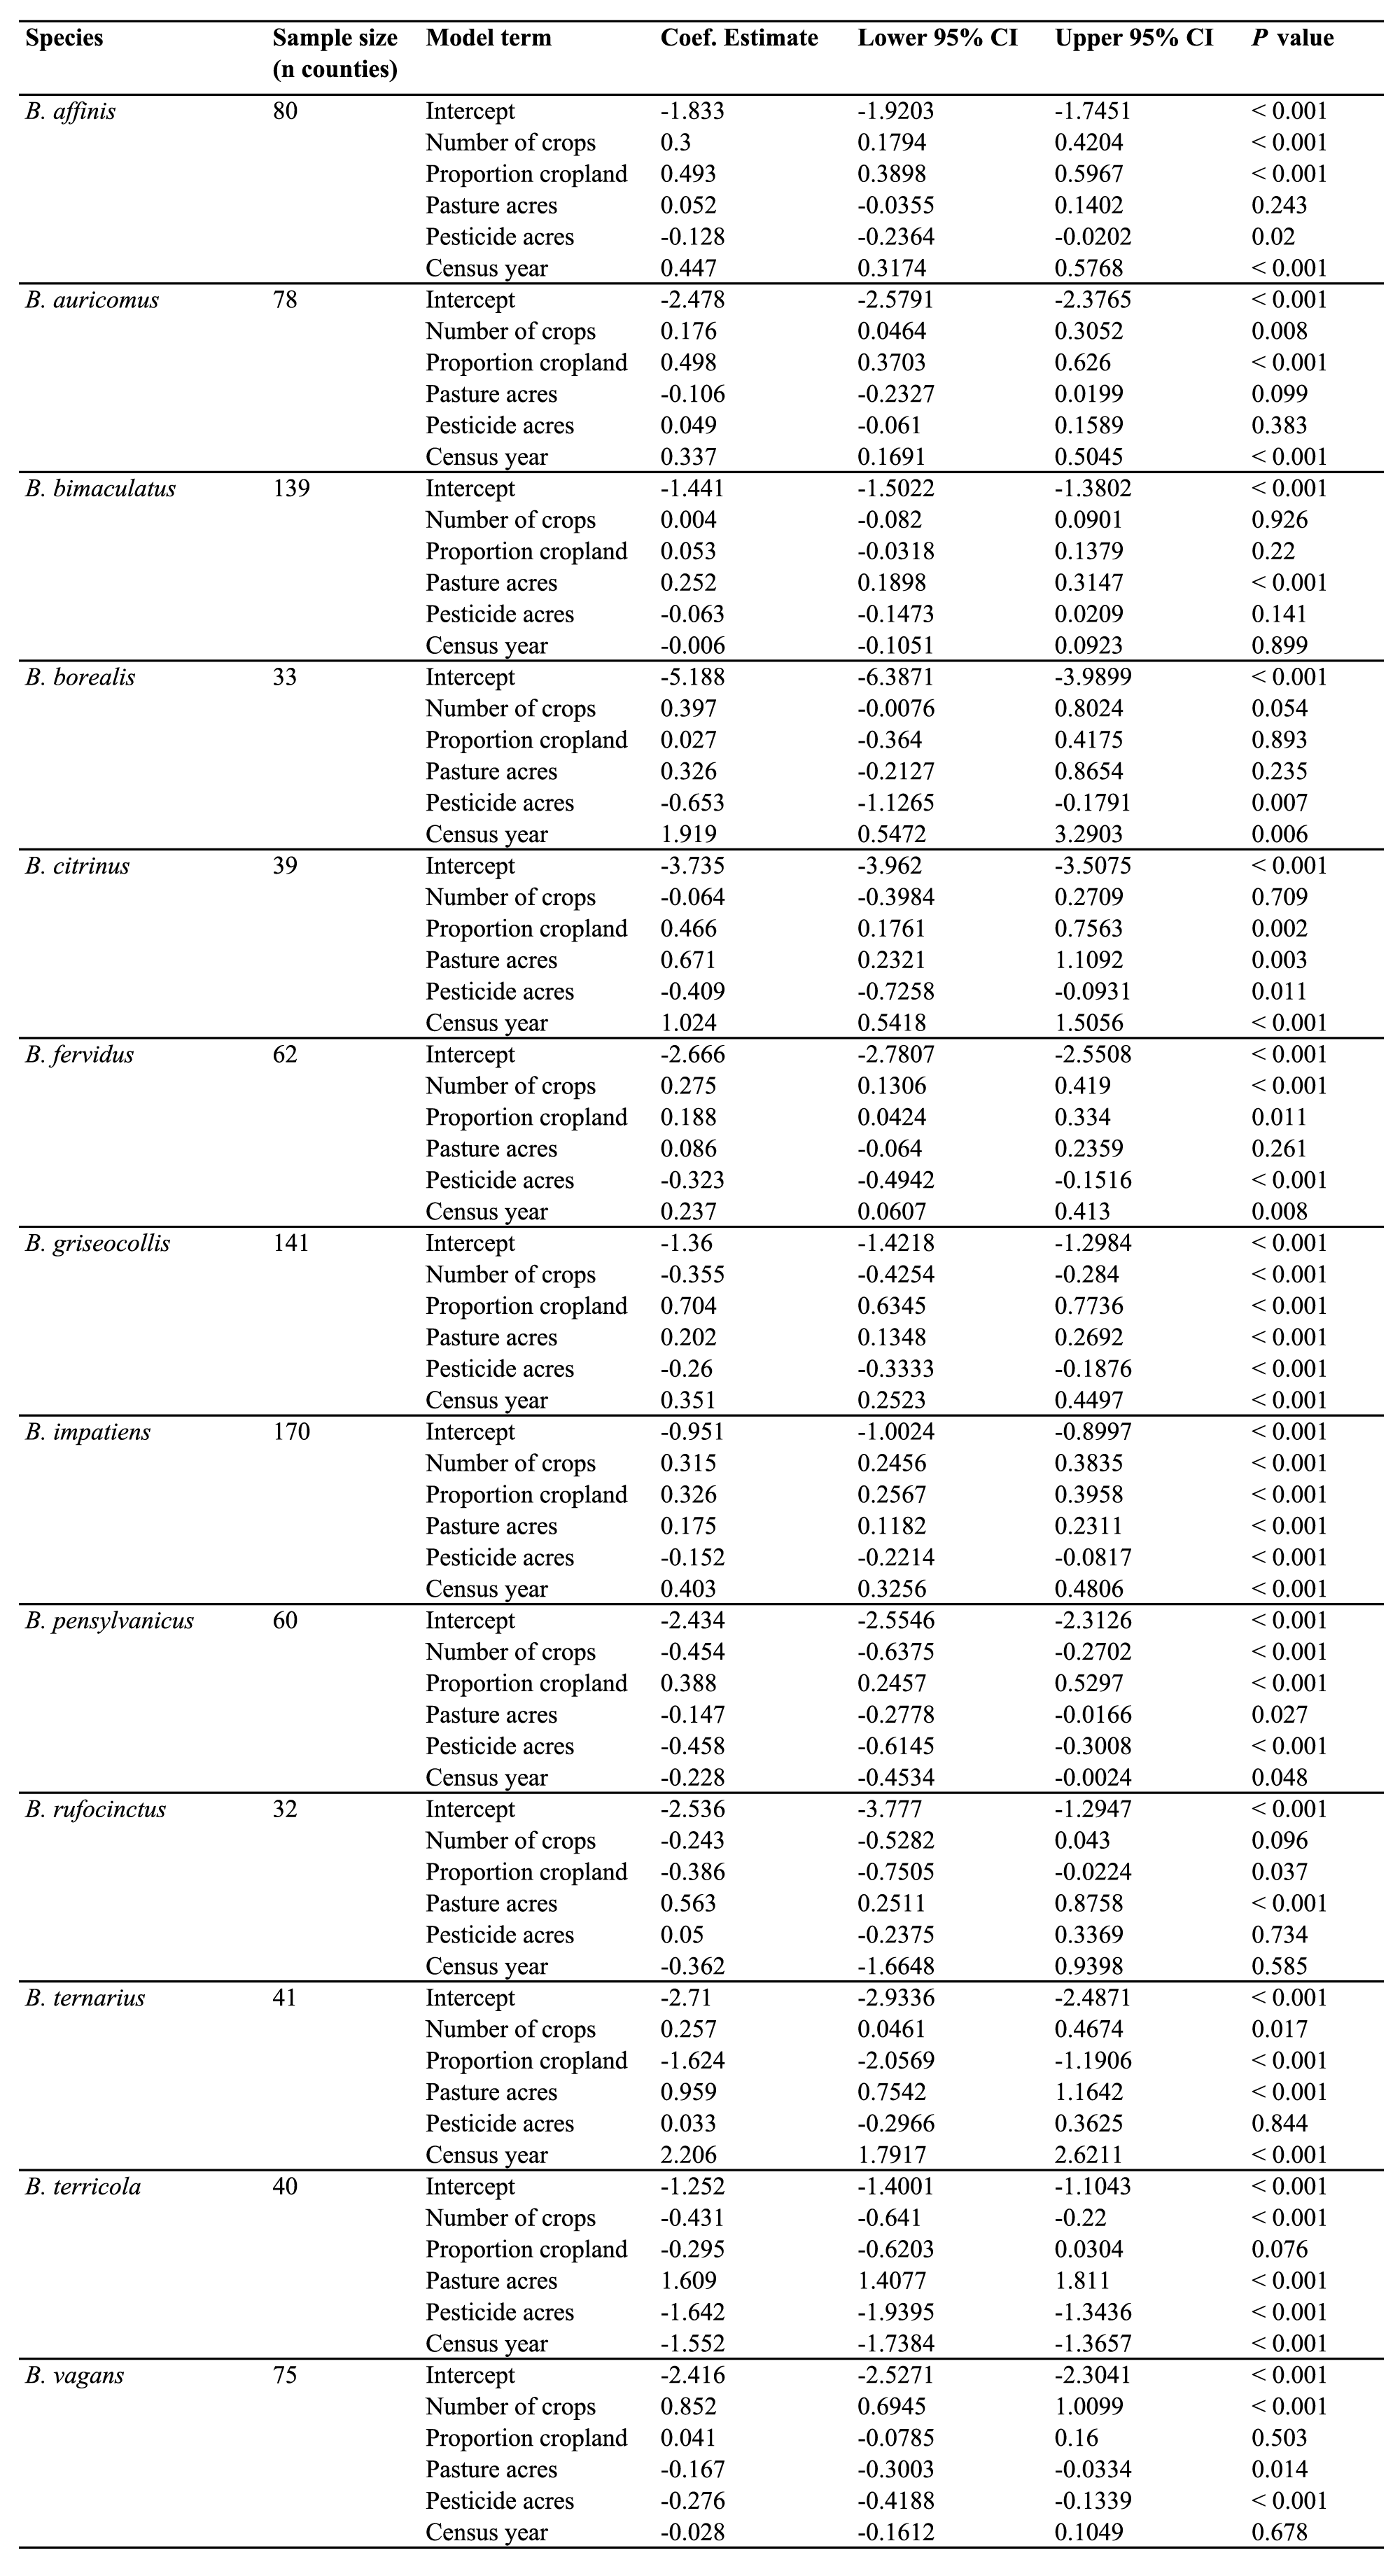
\includegraphics[width=0.6\textwidth,height=\textheight]{../ms_figs/tables2.png}

\clearpage

\newpage

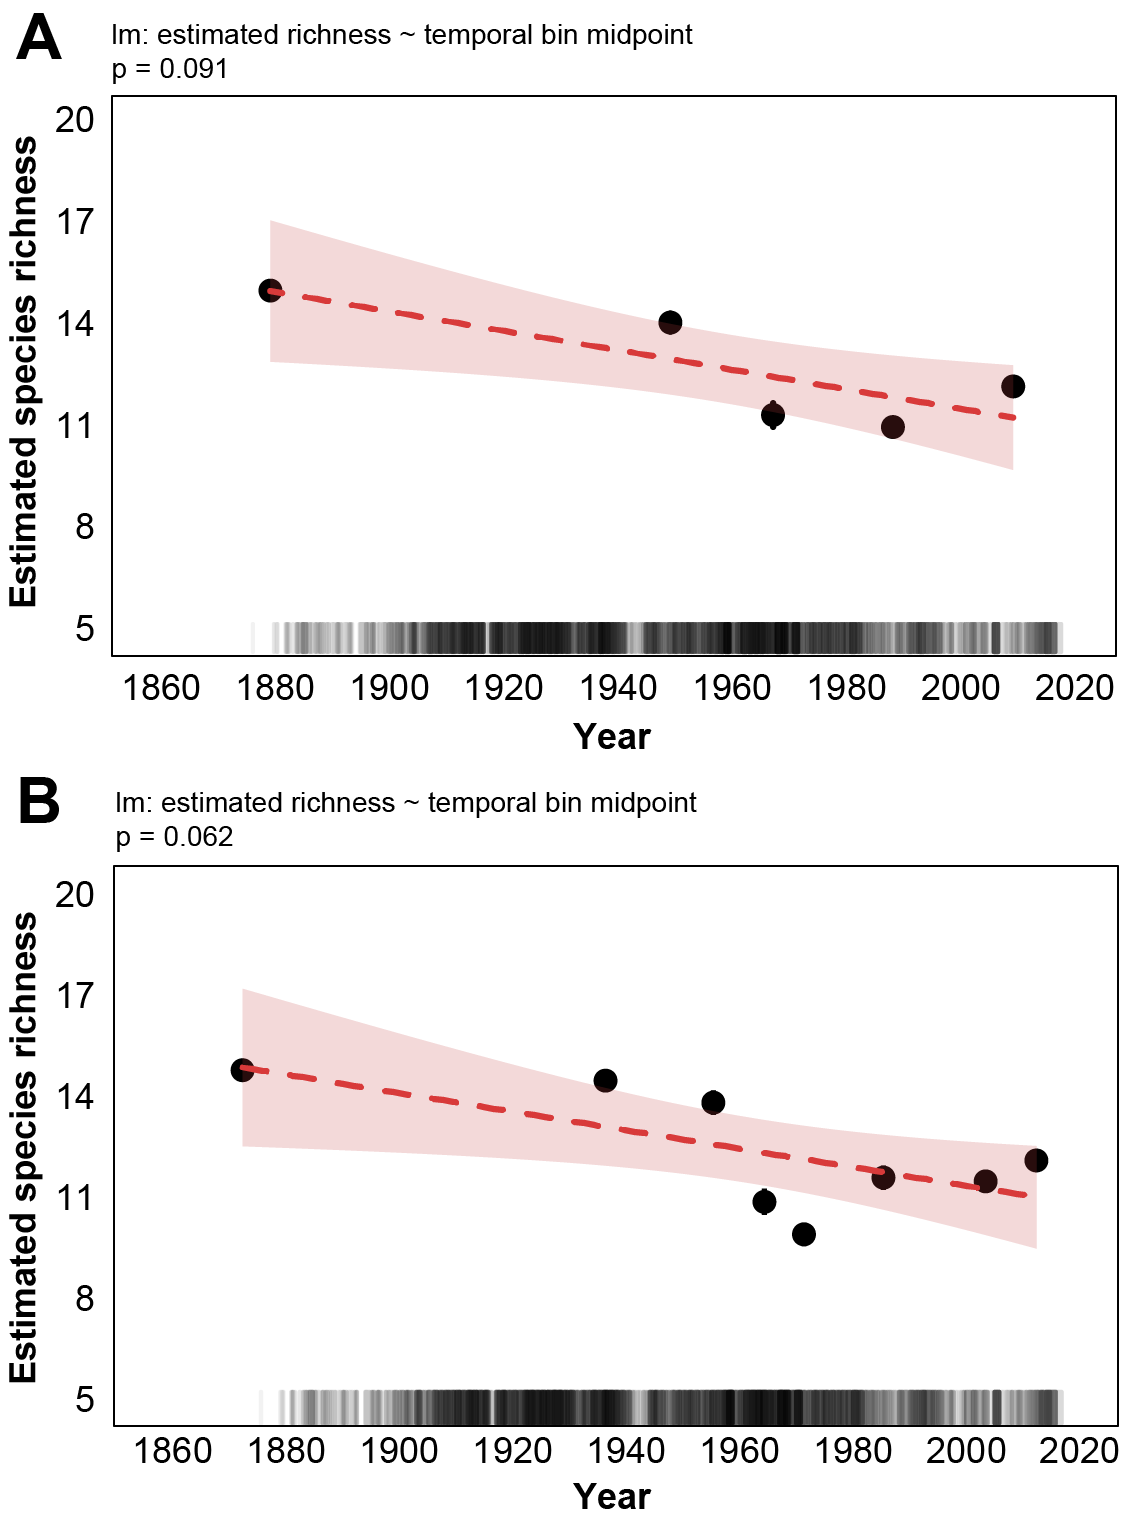
\includegraphics[width=0.6\textwidth,height=\textheight]{../ms_figs/fig_s1.png}

\textbf{Supplementary Figure 1:} Sample-based species accumulation
curves for each of 15 temporal bins (different colors) from which
estimated species richness was calculated (Fig. 1). Each accumulation
curve is constructed for temporal bins with a roughly equal number of
records.

\clearpage

\newpage

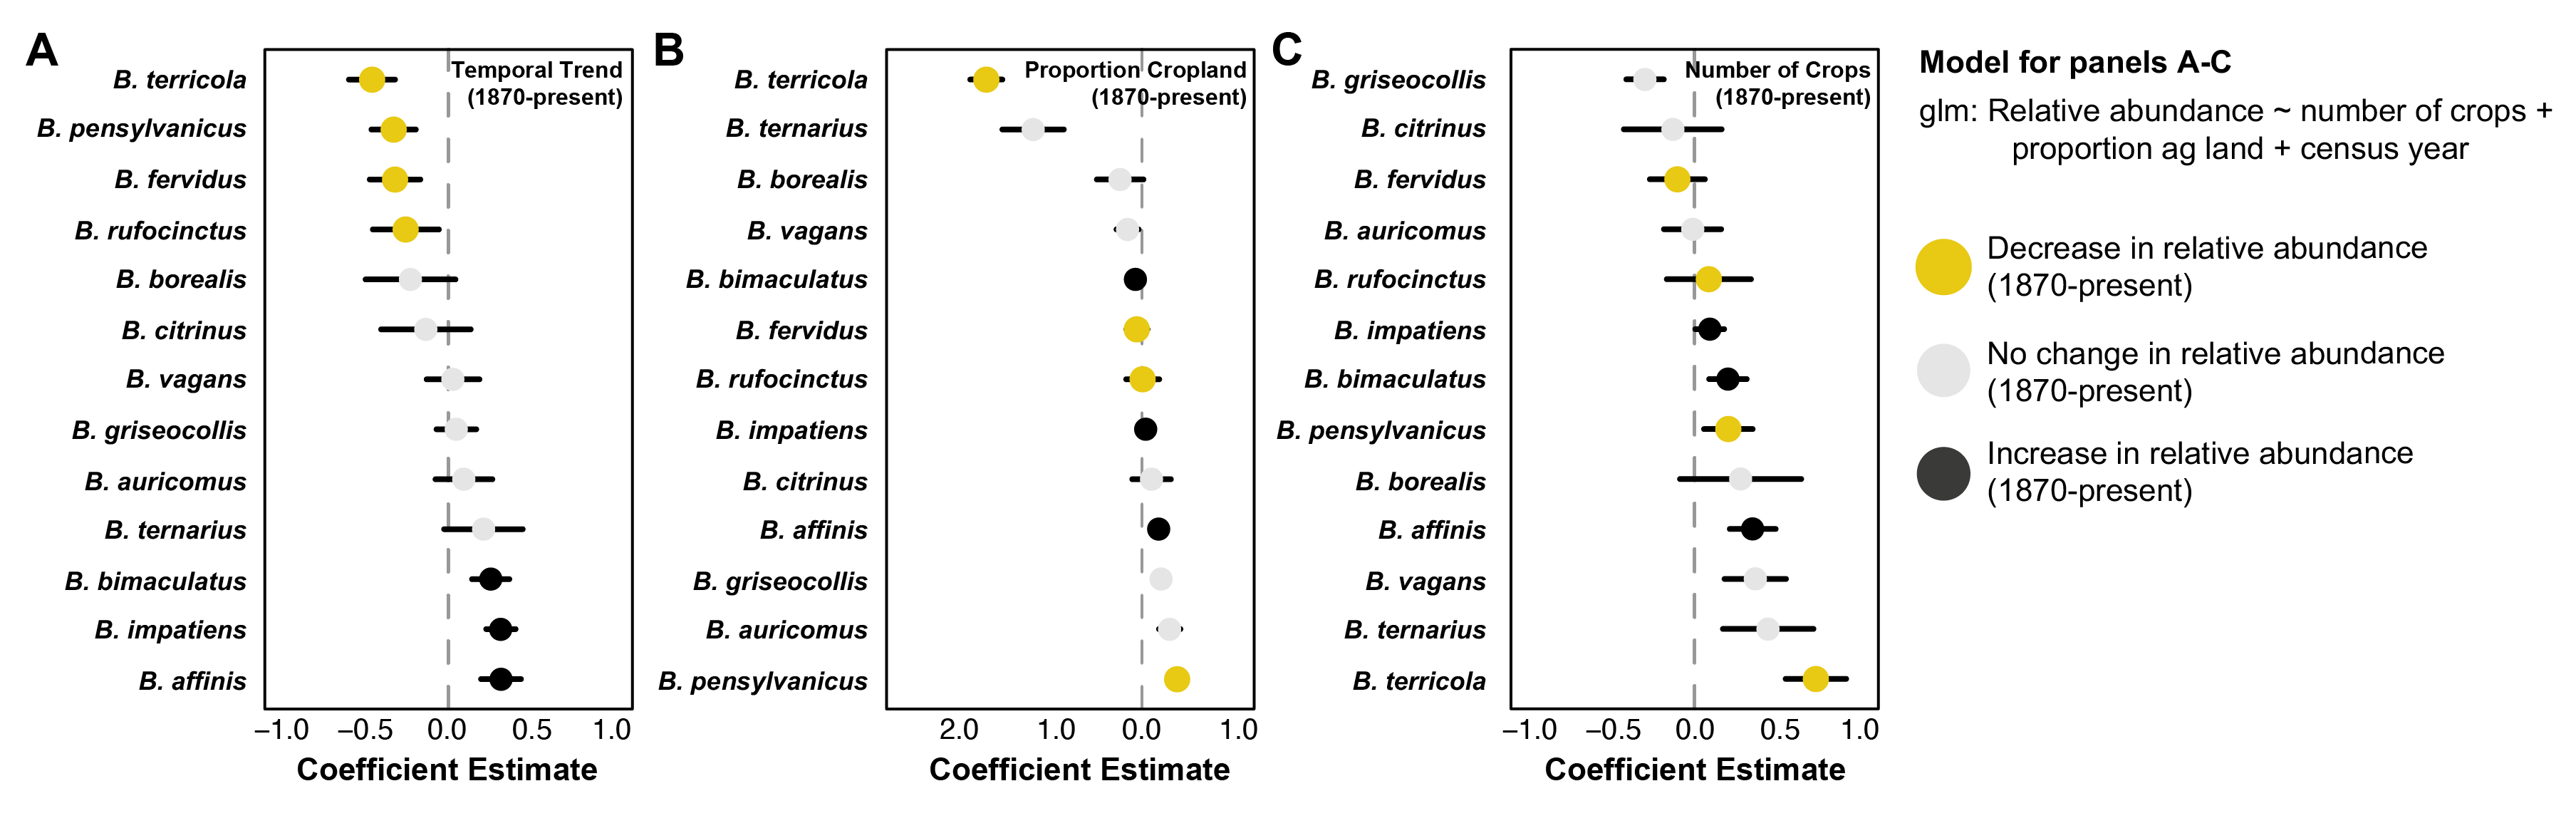
\includegraphics[width=1\textwidth,height=\textheight]{../ms_figs/fig_s2.png}

\textbf{Supplementary Figure 2:} Patterns of agricultural
intensification in two metrics additional metrics from 1982-2012: (a)
total acres of pasture per county and (c) total acreage treated with
insecticides per county. Inset graphs (b,d) depict general trend of
these two variables for each state in the study area as modeled by a
Loess fitted curve. Values beneath years are mean acres ± SEM.

\clearpage

\hypertarget{references}{%
\section*{References}\label{references}}
\addcontentsline{toc}{section}{References}

\hypertarget{refs}{}
\leavevmode\hypertarget{ref-Bartomeus2013}{}%
Bartomeus, Ignasi, Mia G. Park, Jason Gibbs, Bryan N. Danforth, Alan N.
Lakso, and Rachael Winfree. 2013. ``Biodiversity ensures
plant-pollinator phenological synchrony against climate change.''
\emph{Ecol. Lett.} 16 (11): 1331--8.
\url{https://doi.org/10.1111/ele.12170}.

\leavevmode\hypertarget{ref-Bartomeus2019}{}%
Bartomeus, I., J. R. Stavert, D. Ward, and O. Aguado. 2019. ``Historical
collections as a tool for assessing the global pollination crisis.''
\emph{Philos. Trans. R. Soc. B Biol. Sci.} 374 (1763): 1--9.
\url{https://doi.org/10.1098/rstb.2017.0389}.

\leavevmode\hypertarget{ref-Benton2002}{}%
Benton, Tim G., David M. Bryant, Lorna Cole, and Humphrey Q.P. Crick.
2002. ``Linking agricultural practice to insect and bird populations: A
historical study over three decades.'' \emph{J. Appl. Ecol.} 39 (4):
673--87. \url{https://doi.org/10.1046/j.1365-2664.2002.00745.x}.

\leavevmode\hypertarget{ref-Benton2003}{}%
Benton, Tim G., Juliet A. Vickery, and Jeremy D. Wilson. 2003.
``Farmland biodiversity: Is habitat heterogeneity the key?''
\emph{Trends Ecol. Evol.} 18 (4): 182--88.
\url{https://doi.org/10.1016/S0169-5347(03)00011-9}.

\leavevmode\hypertarget{ref-Biesmeijer2006}{}%
Biesmeijer, J. C. 2006. ``Parallel Declines in Pollinators and
Insect-Pollinated Plants in Britain and the Netherlands.'' \emph{Science
(80-. ).} 313 (5785): 351--54.
\url{https://doi.org/10.1126/science.1127863}.

\leavevmode\hypertarget{ref-Brown2000}{}%
Brown, D. G., B. C. Pijanowski, and J. D. Duh. 2000. ``Modeling the
relationships between land use and land cover on private lands in the
Upper Midwest, USA.'' \emph{J. Environ. Manage.} 59 (4): 247--63.
\url{https://doi.org/10.1006/jema.2000.0369}.

\leavevmode\hypertarget{ref-Brown2011}{}%
Brown, Paul W., and Lisa A. Schulte. 2011. ``Agricultural landscape
change (1937-2002) in three townships in Iowa, USA.'' \emph{Landsc.
Urban Plan.} 100 (3): 202--12.
\url{https://doi.org/10.1016/j.landurbplan.2010.12.007}.

\leavevmode\hypertarget{ref-Cameron2011}{}%
Cameron, Sydney A, Jeffrey D Lozier, James P Strange, Jonathan B Koch,
Nils Cordes, Leellen F Solter, Terry L Griswold, and Gene E Robinson.
2011. ``Patterns of widespread decline in North American bumble bees.''
\emph{Proc. Natl. Acad. Sci. U. S. A.} 108 (2): 662--67.
\url{https://doi.org/10.1073/pnas.1014743108}.

\leavevmode\hypertarget{ref-Cane2017}{}%
Cane, James H., and Vincent J. Tepedino. 2017. ``Gauging the Effect of
Honey Bee Pollen Collection on Native Bee Communities.'' \emph{Conserv.
Lett.} 10 (2): 205--10. \url{https://doi.org/10.1111/conl.12263}.

\leavevmode\hypertarget{ref-Carvell2006b}{}%
Carvell, Claire, David B. Roy, Simon M. Smart, Richard F. Pywell, Chris
D. Preston, and Dave Goulson. 2006. ``Declines in forage availability
for bumblebees at a national scale.'' \emph{Biol. Conserv.} 132 (4):
481--89. \url{https://doi.org/10.1016/j.biocon.2006.05.008}.

\leavevmode\hypertarget{ref-Colla2012}{}%
Colla, Sheila R., Fawziah Gadallah, Leif Richardson, David Wagner, and
Lawrence Gall. 2012. ``Assessing declines of North American bumble bees
(Bombus spp.) using museum specimens.'' \emph{Biodivers. Conserv.} 21
(14): 3585--95. \url{https://doi.org/10.1007/s10531-012-0383-2}.

\leavevmode\hypertarget{ref-Colla2008}{}%
Colla, Sheila R., and Laurence Packer. 2008. ``Evidence for decline in
eastern North American bumblebees (Hymenoptera: Apidae), with special
focus on Bombus affinis Cresson.'' \emph{Biodivers. Conserv.}
\url{https://doi.org/10.1007/s10531-008-9340-5}.

\leavevmode\hypertarget{ref-Crall2018}{}%
Crall, James D, Callin M Switzer, Robert L Oppenheimer, Ashlee N. Ford
Versypt, Biswadip Dey, Andrea Brown, Mackay Eyster, et al. 2018.
``Neonicotinoid exposure disrupts bumblebee nest behavior, social
networks, and thermoregulation.'' \emph{Science (80-. ).} 362 (6415):
683--86. \url{https://doi.org/10.1126/science.aat1598}.

\leavevmode\hypertarget{ref-Crone2016}{}%
Crone, Elizabeth E., Neal M. Williams, and Ecology Letters. 2016.
``Bumble bee colony dynamics: Quantifying the importance of land use and
floral resources for colony growth and queen production.'' Edited by
Rebecca Irwin. \emph{Ecol. Lett.} 19 (4): 460--68.
\url{https://doi.org/10.1111/ele.12581}.

\leavevmode\hypertarget{ref-Cusser2018}{}%
Cusser, Sarah, John L. Neff, and Shalene Jha. 2018. ``Land-use history
drives contemporary pollinator community similarity.'' \emph{Landsc.
Ecol.} 33 (8): 1335--51.
\url{https://doi.org/10.1007/s10980-018-0668-2}.

\leavevmode\hypertarget{ref-Dornelas2019}{}%
Dornelas, Maria, Nicholas J. Gotelli, Hideyasu Shimadzu, Faye Moyes,
Anne E. Magurran, and Brian J. McGill. 2019. ``A balance of winners and
losers in the Anthropocene.'' \emph{Ecol. Lett.} 22 (5): 847--54.
\url{https://doi.org/10.1111/ele.13242}.

\leavevmode\hypertarget{ref-Fahrig2011b}{}%
Fahrig, Lenore, Jacques Baudry, Lluís Brotons, Françoise G Burel, Thomas
O Crist, Robert J Fuller, Clelia Sirami, Gavin M Siriwardena, and
Jean-Louis Martin. 2011. ``Functional landscape heterogeneity and animal
biodiversity in agricultural landscapes.'' \emph{Ecol. Lett.} 14 (2):
101--12. \url{https://doi.org/10.1111/j.1461-0248.2010.01559.x}.

\leavevmode\hypertarget{ref-Feltham2014}{}%
Feltham, Hannah, Kirsty Park, and Dave Goulson. 2014. ``Field realistic
doses of pesticide imidacloprid reduce bumblebee pollen foraging
efficiency.'' \emph{Ecotoxicology} 23 (3): 317--23.
\url{https://doi.org/10.1007/s10646-014-1189-7}.

\leavevmode\hypertarget{ref-Fischer2015}{}%
Fischer, Jason D., Sarah C. Schneider, Adam A. Ahlers, and James R.
Miller. 2015. ``Categorizing wildlife responses to urbanization and
conservation implications of terminology.'' \emph{Conserv. Biol.} 29
(4): 1246--8. \url{https://doi.org/10.1111/cobi.12451}.

\leavevmode\hypertarget{ref-Franklin1913}{}%
Franklin, Henry J. 1913. \emph{The Bombidae of the New World}. Vol. 53.
9. {[}Philadelphia{]} : American Entomological Society,
\url{https://doi.org/10.5962/bhl.title.122585}.

\leavevmode\hypertarget{ref-Fye1954a}{}%
Fye, R E, and J T Medler. 1954. ``Spring emergence and floral hosts of
Wisconsin bumblebees.''

\leavevmode\hypertarget{ref-Giles2006}{}%
Giles, Valerie, and JOHN Ascher. 2006. ``A survey of the bees of the
Black Rock Forest preserve, New York (Hymenoptera: Apoidea).'' \emph{J.
Hymenopt. Res.} 15 (2): 208--31.

\leavevmode\hypertarget{ref-Goulson2015c}{}%
Goulson, Dave, Elizabeth Nicholls, C. Botias, Ellen L. Rotheray,
Cristina Botías, and Ellen L. Rotheray. 2015. ``Bee declines driven by
combined stress from parasites, pesticides, and lack of flowers.''
\emph{Science (80-. ).}, no. February: 1--16.
\url{https://doi.org/10.1126/science.1255957}.

\leavevmode\hypertarget{ref-Goulson2005b}{}%
Goulson, D., M. E. Hanley, B. Darvill, J. S. Ellis, and M. E. Knight.
2005. ``Causes of rarity in bumblebees.'' \emph{Biol. Conserv.} 122 (1):
1--8. \url{https://doi.org/10.1016/j.biocon.2004.06.017}.

\leavevmode\hypertarget{ref-Goulson2008c}{}%
Goulson, D, G C Lye, and B Darvill. 2008. ``Decline and conservation of
bumble bees.'' \emph{Annu. Rev. Entomol.} 53 (January): 191--208.
\url{https://doi.org/10.1146/annurev.ento.53.103106.093454}.

\leavevmode\hypertarget{ref-Grixti2009}{}%
Grixti, Jennifer C., Lisa T. Wong, Sydney a. Cameron, and Colin Favret.
2009. ``Decline of bumble bees (Bombus) in the North American Midwest.''
\emph{Biol. Conserv.} 142 (1): 75--84.
\url{https://doi.org/10.1016/j.biocon.2008.09.027}.

\leavevmode\hypertarget{ref-Hallmann2017}{}%
Hallmann, Caspar A., Martin Sorg, Eelke Jongejans, Henk Siepel, Nick
Hofland, Heinz Schwan, Werner Stenmans, et al. 2017. ``More than 75
percent decline over 27 years in total flying insect biomass in
protected areas.'' \emph{PLoS One} 12 (10): e0185809.
\url{https://doi.org/10.1371/journal.pone.0185809}.

\leavevmode\hypertarget{ref-Hass2018a}{}%
Hass, Annika Louise, Lara Brachmann, Péter Batáry, Yann Clough, Hermann
Behling, and Teja Tscharntke. 2018. ``Maize-dominated landscapes reduce
bumblebee colony growth through pollen diversity loss.'' \emph{J. Appl.
Ecol.}, no. September: 1--11.
\url{https://doi.org/10.1111/1365-2664.13296}.

\leavevmode\hypertarget{ref-Hemberger2018}{}%
Hemberger, Jeremy, and Claudio Gratton. 2018. ``Floral resource pulse
decreases bumble bee foraging trip duration in central Wisconsin
agroecosystem.'' \emph{Ecol. Entomol.} 43 (4): 447--57.
\url{https://doi.org/10.1111/een.12516}.

\leavevmode\hypertarget{ref-Hsieh2016}{}%
Hsieh, T. C., K. H. Ma, and Anne Chao. 2016. ``iNEXT: an R package for
rarefaction and extrapolation of species diversity (Hill numbers).''
\emph{Methods Ecol. Evol.} 7 (12): 1451--6.
\url{https://doi.org/10.1111/2041-210X.12613}.

\leavevmode\hypertarget{ref-Jacobson2018a}{}%
Jacobson, Molly M., Erika M. Tucker, Minna E. Mathiasson, and Sandra M.
Rehan. 2018. ``Decline of bumble bees in northeastern North America,
with special focus on Bombus terricola.'' \emph{Biol. Conserv.} 217
(August 2017): 437--45.
\url{https://doi.org/10.1016/j.biocon.2017.11.026}.

\leavevmode\hypertarget{ref-Kerr2015}{}%
Kerr, Jeremy T, Alana Pindar, Paul Galpern, Laurence Packer, Simon G
Potts, Stuart M Roberts, Pierre Rasmont, et al. 2015. ``Climate change
impacts on bumblebees converge across continents.'' \emph{Science (80-.
).} 349 (6244): 177--80. \url{https://doi.org/10.1126/science.aaa7031}.

\leavevmode\hypertarget{ref-Kleijn2008}{}%
Kleijn, David, and Ivo Raemakers. 2008. ``A retrospective analysis of
pollen host plant use by stable and declining bumble bee species.''
\emph{Ecology} 89 (7): 1811--23.
\url{https://doi.org/10.1890/07-1275.1}.

\leavevmode\hypertarget{ref-Klein2007g}{}%
Klein, Alexandra-Maria, Bernard E Vaissière, James H Cane, Ingolf
Steffan-Dewenter, Saul a Cunningham, Claire Kremen, and Teja Tscharntke.
2007. ``Importance of pollinators in changing landscapes for world
crops.'' \emph{Proc. Biol. Sci.} 274 (1608): 303--13.
\url{https://doi.org/10.1098/rspb.2006.3721}.

\leavevmode\hypertarget{ref-Kremen2002}{}%
Kremen, Claire, Neal M Williams, and Robbin W Thorp. 2002. ``Crop
pollination from native bees at risk from agricultural
intensification.'' \emph{Proc. Natl. Acad. Sci. U. S. A.} 99 (26):
16812--6. \url{https://doi.org/10.1073/pnas.262413599}.

\leavevmode\hypertarget{ref-Landis2017}{}%
Landis, Douglas A. 2017. ``Designing agricultural landscapes for
biodiversity-based ecosystem services.'' \emph{Basic Appl. Ecol.} 18:
1--12. \url{https://doi.org/10.1016/j.baae.2016.07.005}.

\leavevmode\hypertarget{ref-Mallinger2017a}{}%
Mallinger, Rachel E, Hannah R. Gaines-Day, and Claudio Gratton. 2017.
``Do managed bees have negative effects on wild bees?: A systematic
review of the literature.'' Edited by Nigel E. Raine. \emph{PLoS One} 12
(12): e0189268. \url{https://doi.org/10.1371/journal.pone.0189268}.

\leavevmode\hypertarget{ref-Marshall2017}{}%
Marshall, Leon, Jacobus C. Biesmeijer, Pierre Rasmont, Nicolas J.
Vereecken, Libor Dvorak, Una Fitzpatrick, Frédéric Francis, et al. 2017.
``The interplay of climate and land use change affects the distribution
of EU bumblebees.'' \emph{Glob. Chang. Biol.}, no. July: 1--16.
\url{https://doi.org/10.1111/gcb.13867}.

\leavevmode\hypertarget{ref-McArt2017}{}%
McArt, Scott H., Christine Urbanowicz, Shaun McCoshum, Rebecca E. Irwin,
and Lynn S. Adler. 2017. ``Landscape predictors of pathogen prevalence
and range contractions in US bumblebees.'' \emph{Proc. R. Soc. B Biol.
Sci.} 284 (1867): 20172181.
\url{https://doi.org/10.1098/rspb.2017.2181}.

\leavevmode\hypertarget{ref-McKinney1999}{}%
McKinney, Ml, and Jl Lockwood. 1999. ``Biotic homogenization: a few
winners replacing many losers in the next mass extinction.''
\emph{Trends Ecol. Evol.} 14 (11): 450--53.
\url{http://www.ncbi.nlm.nih.gov/pubmed/10511724}.

\leavevmode\hypertarget{ref-Meehan2015}{}%
Meehan, Timothy D., and Claudio Gratton. 2015. ``A consistent positive
association between landscape simplification and insecticide use across
the Midwestern US from 1997 through 2012.'' \emph{Environ. Res. Lett.}
10 (11). \url{https://doi.org/10.1088/1748-9326/10/11/114001}.

\leavevmode\hypertarget{ref-Meehan2010a}{}%
Meehan, Timothy D, Allen H Hurlbert, and Claudio Gratton. 2010. ``Bird
communities in future bioenergy landscapes of the Upper Midwest.''
\emph{Proc. Natl. Acad. Sci. U. S. A.} 107 (43): 18533--8.
\url{https://doi.org/10.1073/pnas.1008475107}.

\leavevmode\hypertarget{ref-Meehan2011}{}%
Meehan, Timothy D, Ben P Werling, Douglas a Landis, and Claudio Gratton.
2011. ``Agricultural landscape simplification and insecticide use in the
Midwestern United States.'' \emph{Proc. Natl. Acad. Sci. U. S. A.} 108
(28): 11500--11505. \url{https://doi.org/10.1073/pnas.1100751108}.

\leavevmode\hypertarget{ref-Morales2013}{}%
Morales, Carolina L., Marina P. Arbetman, Sydney A. Cameron, and Marcelo
A. Aizen. 2013. ``Rapid ecological replacement of a native bumble bee by
invasive species.'' \emph{Front. Ecol. Environ.} 11 (10): 529--34.
\url{https://doi.org/10.1890/120321}.

\leavevmode\hypertarget{ref-Ollerton2011}{}%
Ollerton, Jeff, Rachael Winfree, and Sam Tarrant. 2011. ``How many
flowering plants are pollinated by animals?'' \emph{Oikos} 120 (3):
321--26. \url{https://doi.org/10.1111/j.1600-0706.2010.18644.x}.

\leavevmode\hypertarget{ref-Pearce2006}{}%
Pearce, Jennie L., and Mark S. Boyce. 2006. ``Modelling distribution and
abundance with presence-only data.'' \emph{J. Appl. Ecol.} 43 (3):
405--12. \url{https://doi.org/10.1111/j.1365-2664.2005.01112.x}.

\leavevmode\hypertarget{ref-Rasmont2012}{}%
Rasmont, Pierre, and Stéphanie Iserbyt. 2012. ``The bumblebees scarcity
syndrome: Are heat waves leading to local extinctions of bumblebees
(Hymenoptera: Apidae: Bombus)?'' \emph{Ann. La Soc. Entomol. Fr.} 48
(3-4): 275--80. \url{https://doi.org/10.1080/00379271.2012.10697776}.

\leavevmode\hypertarget{ref-Rhemtulla2007a}{}%
Rhemtulla, Jeanine M., David J. Mladenoff, and Murray K. Clayton. 2007.
``Regional land-cover conversion in the U.S. upper Midwest: Magnitude of
change and limited recovery (1850-1935-1993).'' \emph{Landsc. Ecol.} 22
(SUPPL. 1): 57--75. \url{https://doi.org/10.1007/s10980-007-9117-3}.

\leavevmode\hypertarget{ref-Richardson2018}{}%
Richardson, L.L, K.P McFarland, S Zahendra, and S Hardy. 2018. ``Bumble
bee (\textless{}i\textgreater{}Bombus\textless{}/i\textgreater{})
distribution and diversity in Vermont, USA: A century of change.''
\emph{J. Insect Conserv.} In Review (0): 0.
\url{https://doi.org/10.1007/s10841-018-0113-5}.

\leavevmode\hypertarget{ref-Ropars2019}{}%
Ropars, Lise, Isabelle Dajoz, Colin Fontaine, Audrey Muratet, and Benoît
Geslin. 2019. ``Wild pollinator activity negatively related to honey bee
colony densities in urban context.'' Edited by Wolfgang Blenau.
\emph{PLoS One} 14 (9): e0222316.
\url{https://doi.org/10.1371/journal.pone.0222316}.

\leavevmode\hypertarget{ref-Schellhorn2015c}{}%
Schellhorn, Nancy A., Vesna Gagic, and Riccardo Bommarco. 2015. ``Time
will tell: Resource continuity bolsters ecosystem services.''
\emph{Trends Ecol. Evol.} 30 (9): 524--30.
\url{https://doi.org/10.1016/j.tree.2015.06.007}.

\leavevmode\hypertarget{ref-Schmid-Hempel1998a}{}%
Schmid-Hempel, Regula, and Paul Schmid-Hempel. 1998. ``Colony
performance and immunocompetence of a social insect, Bombus terrestris,
in poor and variable environments.'' \emph{Funct. Ecol.} 12 (1): 22--30.
\url{https://doi.org/10.1046/j.1365-2435.1998.00153.x}.

\leavevmode\hypertarget{ref-Seibold2019}{}%
Seibold, Sebastian, Martin M Gossner, Nadja K Simons, Nico Blüthgen,
Didem Ambarl, Christian Ammer, Jürgen Bauhus, et al. 2019. ``Arthropod
decline in grasslands and forests is associated with drivers at
landscape level.'' \emph{Nature} 574 (February): 1--34.
\url{https://doi.org/10.1038/s41586-019-1684-3}.

\leavevmode\hypertarget{ref-Sirami2019}{}%
Sirami, Clélia, Nicolas Gross, Aliette Bosem Baillod, Colette Bertrand,
Romain Carrié, Annika Hass, Laura Henckel, et al. 2019. ``Increasing
crop heterogeneity enhances multitrophic diversity across agricultural
regions.'' \emph{Proc. Natl. Acad. Sci.}, July, 201906419.
\url{https://doi.org/10.1073/pnas.1906419116}.

\leavevmode\hypertarget{ref-Sirois-Delisle2018}{}%
Sirois-Delisle, Catherine, and Jeremy T. Kerr. 2018. ``Climate
change-driven range losses among bumblebee species are poised to
accelerate.'' \emph{Sci. Rep.} 8 (1): 14464.
\url{https://doi.org/10.1038/s41598-018-32665-y}.

\leavevmode\hypertarget{ref-Smith1998}{}%
Smith, Daryl D. 1998. ``Iowa prairie: Original extent and loss,
preservation and recovery attempts.'' \emph{J. Iowa Acad. Sci.} 105 (3):
94--108.

\leavevmode\hypertarget{ref-Steffan-Dewenter2005c}{}%
Steffan-Dewenter, Ingolf, Simon G. Potts, Laurence Packer, and Jaboury
Ghazoul. 2005. ``Pollinator diversity and crop pollination services are
at risk {[}3{]} (multiple letters).'' \emph{Trends Ecol. Evol.} 20 (12):
651--53. \url{https://doi.org/10.1016/j.tree.2005.09.004}.

\leavevmode\hypertarget{ref-Torne-Noguera2016}{}%
Torné-Noguera, Anna, Anselm Rodrigo, Sergio Osorio, and Jordi Bosch.
2016. ``Collateral effects of beekeeping: Impacts on pollen-nectar
resources and wild bee communities.'' \emph{Basic Appl. Ecol.} 17 (3):
199--209. \url{https://doi.org/10.1016/j.baae.2015.11.004}.

\leavevmode\hypertarget{ref-Turner2012}{}%
Turner, Monica G., Daniel C. Donato, and William H. Romme. 2012.
``Consequences of spatial heterogeneity for ecosystem services in
changing forest landscapes: priorities for future research.''
\emph{Landsc. Ecol.} 28 (6): 1081--97.
\url{https://doi.org/10.1007/s10980-012-9741-4}.

\leavevmode\hypertarget{ref-Vaudo2015}{}%
Vaudo, Anthony D., John F. Tooker, Christina M. Grozinger, and Harland
M. Patch. 2015. ``Bee nutrition and floral resource restoration.''
\emph{Curr. Opin. Insect Sci.} 10: 133--41.
\url{https://doi.org/10.1016/j.cois.2015.05.008}.

\leavevmode\hypertarget{ref-Westphal2009a}{}%
Westphal, C., I. Steffan-Dewenter, and T. Tscharntke. 2009. ``Mass
flowering oilseed rape improves early colony growth but not sexual
reproduction of b1. Westphal, C., Steffan-Dewenter, I. \& Tscharntke, T.
(2009). Mass flowering oilseed rape improves early colony growth but not
sexual reproduction of bumblebees. J.'' \emph{J. Appl. Ecol.} 46 (1):
187--93. \url{https://doi.org/10.1111/j.1365-2664.2008.01580.x}.

\leavevmode\hypertarget{ref-Whitehorn2012}{}%
Whitehorn, Penelope R., Stephanie O'Connor, Felix L. Wackers, and Dave
Goulson. 2012. ``Neonicotinoid Pesticide Reduces Bumble Bee Colony
Growth and Queen Production.'' \emph{Science (80-. ).} 336 (6079):
351--52. \url{https://doi.org/10.1126/science.1215025}.

\leavevmode\hypertarget{ref-Williams2012b}{}%
Williams, Neal M., James Regetz, and Claire Kremen. 2012.
``Landscape-scale resources promote colony growth but not reproductive
performance of bumble bees.'' \emph{Ecology} 93 (5): 1049--58.
\url{https://doi.org/10.1890/11-1006.1}.

\leavevmode\hypertarget{ref-Williams1986}{}%
Williams, Paul H. 1986. ``Environmental change and the distributions of
british bumble bees (bombus latr.).'' \emph{Bee World} 67 (2): 50--61.
\url{https://doi.org/10.1080/0005772X.1986.11098871}.

\leavevmode\hypertarget{ref-Williams2007}{}%
Williams, Paul H., Miguel B. Araújo, and Pierre Rasmont. 2007. ``Can
vulnerability among British bumblebee (Bombus) species be explained by
niche position and breadth?'' \emph{Biol. Conserv.} 138 (3-4): 493--505.
\url{https://doi.org/10.1016/j.biocon.2007.06.001}.

\leavevmode\hypertarget{ref-Williams2009}{}%
Williams, Paul, and Juliet L Osborne. 2009. ``Bumblebee vulnerability
and conservation world-wide.'' \emph{Apidologie} 40: 367--87.

\leavevmode\hypertarget{ref-Wood2019}{}%
Wood, Thomas J., Jason Gibbs, Kelsey K. Graham, and Rufus Isaacs. 2019.
``Narrow pollen diets are associated with declining Midwestern bumble
bee species.'' \emph{Ecology} 0 (0).
\url{https://doi.org/10.1002/ecy.2697}.

\leavevmode\hypertarget{ref-Woodard2017a}{}%
Woodard, S. Hollis. 2017. ``Bumble bee ecophysiology: integrating the
changing environment and the organism.'' \emph{Curr. Opin. Insect Sci.}
22: 101--8. \url{https://doi.org/10.1016/j.cois.2017.06.001}.


\end{document}
